\documentclass[12pt,a4paper,twoside,openright]{book}

\usepackage[italian]{babel}
\usepackage{style/isi-lt}

% ! TeX root = ../bachelor-thesis.tex

\definecolor{dkgreen}{rgb}{0,0.6,0}
\definecolor{gray}{rgb}{0.5,0.5,0.5}
\definecolor{mauve}{rgb}{0.58,0,0.82}

\lstset{
  frame=single,
  captionpos=b,
  language=Java,
  aboveskip=3mm,
  belowskip=3mm,
  showstringspaces=false,
  columns=flexible,
  basicstyle={\small\ttfamily},
  numbers=none,
  numberstyle=\tiny\color{gray},
  keywordstyle=\color{blue},
  commentstyle=\color{dkgreen},
  stringstyle=\color{mauve},
  breaklines=true,
  breakatwhitespace=true,
  tabsize=3
}
%--------------------------------------------------------------------
%---------------------- INFORMAZIONI SULLA TESI ---------------------
%--------------------------------------------------------------------

\universita{Alma Mater Studiorum -- Università di Bologna}
\campus{Campus di Cesena}
\dipartimento{Dipartimento di Informatica -- Scienza e Ingegneria}
\cdl{Corso di Laurea in Ingegneria e Scienze Informatiche}

\titolo{PROGETTAZIONE E SVILUPPO DI UN SISTEMA DOMOTICO
INTEGRATO CON ASSISTENTE VOCALE A SUPPORTO
DI SERVIZI SOCIO-ASSISTENZIALI BASATI SU GAMIFICATION}
\materia{Sistemi Embedded e Internet Of Things}

\laureando{Jahrim Gabriele Cesario}

\relatore[Prof.]{Alessandro Ricci}
\correlatorea[Ing.]{Massimiliano Malavasi}
\correlatoreb[Dott.ssa]{Laura Bugo}

\annoaccademico{2020 -- 2021}

\makeindex

\begin{document}
\frontmatter

\maketitle
\tableofcontents

% ! TeX root = ../bachelor-thesis.tex

\chapter{Introduzione}

L’uomo ha da sempre cercato di sopperire ai propri limiti, inventando e
costruendo strumenti che lo aiutassero nel soddisfare i propri bisogni di
libertà. Recentemente, uno di questi strumenti è stato la domotica, che, tra le
altre cose, si propone di facilitare la vita in ambito domestico, permettendo
di velocizzare o addirittura automatizzare, quelle piccole azioni quotidiane
che possono rubare via del tempo, oggi più che mai prezioso. Non è tutto però.
Infatti è proprio attraverso la domotica che molte persone ora vedono davanti a
sé una prospettiva d'indipendenza, nella quale quelle azioni quotidiane, prima
per loro impraticabili, diventano finalmente accessibili.

Con il passare del tempo, l’accessibilità ha acquisito sempre maggiore
importanza. Più precisamente, per accessibilità s’intende la capacità di un
servizio di essere fruibile dal maggior numero di persone possibile.
L’accessibilità è quindi cruciale per includere le persone, ma anche per
assicurare il nostro futuro. Infatti, man mano che si invecchia, sempre più
strumenti diventano sempre meno accessibili.

Ormai la domotica è un concetto ben consolidato e sta cominciando a diffondersi
su larga scala, permeando nelle case delle persone, a cui sta diventando sempre
più familiare. Per questo motivo, si presta come ottimo punto di appoggio per
lo sviluppo di servizi integrativi, che possano estendere le funzionalità del
proprio sistema domotico.

In questo contesto, in collaborazione con la AUSL \cite{AUSL} e il CRA
\cite{CRA} di Bologna, sotto la guida del coordinatore del CRA \textit{Ing.
Massimiliano Malavasi}, la neuropsicologa \textit{Dott.ssa Arianna Gherardini}
e la sviluppatrice software \textit{Dott.ssa Laura Bugo}, si è pensato di
progettare un servizio integrativo a un impianto domotico, che consenta di
mantenere in allenamento le proprie capacità cognitive, oltre a fornire
assistenza nello svolgimento delle attività di vita quotidiana. Questa suite è
stata pensata soprattutto come supporto per gli anziani o per le persone con
difficoltà cognitive, ma potrà anche svolgere una funzione di agevolazione e
intrattenimento per i giovani. Più in particolare, si vorrebbe applicare la
suite a un contesto socio-sanitario per assistere persone con disabilità e/o
con difficoltà cognitive e monitorarne i progressi durante il loro percorso
psico-educativo, sotto la supervisione di personale qualificato. La suite
prevederà anche un’assistente vocale che avrà sia la funzione di aumentare
l’accessibilità dell’impianto domotico, sia di permettere l’accesso al servizio
integrativo.

Questa tesi illustrerà come è stato sviluppato questo progetto dalla fase di
analisi del problema fino ai primi risultati prodotti. Sarà quindi descritta
una panoramica generale dei concetti necessari a comprendere le tecnologie
coinvolte e l’obiettivo preposto. Successivamente, sarà analizzato il problema,
delineando quelli che saranno i requisiti del sistema. Sarà poi proposta una
possibile soluzione concettuale, non vincolata a dei servizi specifici, che
descriverà la natura del problema. A questa seguirà una soluzione concreta,
basata su servizi oggi esistenti, di cui se ne motiverà l’adeguatezza,
illustrandone vantaggi e svantaggi. Infine, sarà presentata l'implementazione
di un prototipo e commentati i risultati dei test eseguiti durante la fase di
validazione.


\mainmatter

\pagestyle{fancy}
\fancyhead[LE,RO]{\thepage}
\fancyfoot{}

% ! TeX root = ../bachelor-thesis.tex

\chapter{Definizione del problema}
\label{ch:Chapter1}

In questo capitolo, sarà introdotto lo scopo del progetto e saranno illustrati
i concetti fondamentali che consentiranno al lettore di comprendere a pieno
l’obiettivo del progetto e le tecnologie utilizzate per realizzarlo.

\section{Scopo del progetto}
\label{sec:Sezione1.1}

Questo progetto nasce con lo scopo di assistere persone anziane, fragili o con
disabilità, permettendo loro di ottenere una certa indipendenza nello svolgere
le azioni quotidiane in ambito domestico. Inoltre, si propone di fornire un
servizio integrativo per poter mantenere in allenamento le proprie capacità
cognitive. Questo servizio potrà essere utilizzato anche in un contesto
socio-sanitario, dagli operatori competenti, per realizzare un percorso
educativo per pazienti con difficoltà cognitive e monitorarne i progressi, così
da tenere traccia dei miglioramenti ottenuti.

L’idea è quella d'integrare un’assistente vocale a un sistema domotico, creando
una suite che comprenderà i servizi di entrambi. Nello specifico, il
\textit{sistema domotico} si occuperà di agevolare la vita domestica degli
utenti, rendendo più accessibili gli strumenti di uso quotidiano, come porte e
finestre. L’\textit{assistente vocale} fornirà invece un supporto al sistema
domotico, permettendo di controllarlo tramite comandi vocali, ma consentirà
anche di accedere agli esercizi cognitivi di cui è composto il servizio
integrativo, che si baserà perciò su interazioni prettamente vocali. Per gli
esercizi cognitivi, si è pensato di progettare dei giochi che richiedano
l’impiego di alcune funzioni cognitive del cervello, seguendo i principi di
\textit{gamification}. In questo modo, si rende il servizio più accattivante,
stimolando l'utente all'utilizzo dello stesso.

\section{Contesto}
\label{sec:Sezione1.2}

Di seguito sarà contestualizzato il progetto, approfondendo i concetti che sono
stati utilizzati per descriverlo.

In particolare, si introdurrà la domotica, distinguendo il concetto d'impianto
domotico da quello di \textit{smart home} e descrivendo alcuni degli approcci
usati per controllare un sistema domotico. Seguirà poi, una breve storia sullo
sviluppo degli assistenti vocali e delle funzioni che ricoprono oggigiorno.
Infine, saranno illustrate le capacità cognitive del cervello, in modo da poter
comprendere come il servizio che si vuole progettare possa esercitarle, dunque
mantenendole in allenamento.

\subsection{La domotica}
\label{subsec:Sezione1.2.1}

Il termine \textit{domotica} \cite{DOMOTIC_SYSTEM} deriva dal latino
\textit{domus}, ovvero \textit{casa}, e dal suffisso greco \textit{-ticos}, che
indica le discipline che si applicano a un determinato concetto. Nello
specifico, il termine indica la scienza che studia e applica delle tecnologie
adatte a migliorare la qualità della vita in ambiente domestico.

L’applicazione della domotica si manifesta spesso sotto forma di un impianto
domotico. Un impianto domotico è l’insieme composto da alcuni dispositivi
elettronici e dell’infrastruttura che questi utilizzano per comunicare tra di
loro (un esempio, è l’impianto \textit{KNX} \cite{KONNEX}). Un dispositivo
domotico è infatti uno strumento non più solo passivo, ovvero che subisce
solamente le sollecitazioni dall’ambiente esterno, ma ha anche una parte
attiva, che processa tali sollecitazioni e le trasmette come eventi
identificabili e recepibili da altri strumenti. In questo modo, si crea un
organismo di strumenti che producono eventi e che possono reagire ad alcuni di
essi, modificando lo stato in cui si trovano.

I costi di un impianto domotico sono piuttosto ingenti e dipendono in parte dai
dispositivi da acquistare, ma soprattutto dalla progettazione e installazione
dell’infrastruttura su cui comunicheranno. Per questo, oggi la domotica si
manifesta molto più comunemente sotto forma di \textbf{\textit{smart home}}
(Figura \ref{fig:figure1.1}). Una \textit{smart home} è simile a un impianto
domotico, ma non necessita dell’installazione di un’infrastruttura ad hoc,
infatti ne utilizza una preesistente: Internet. I dispositivi che ricevono e
trasmettono eventi attraverso una connessione a Internet prendono il nome di
dispositivi smart, e sono alla base dell’\textbf{\textit{Internet Of Things}}.

\begin{figure}[!ht]
  \centering
  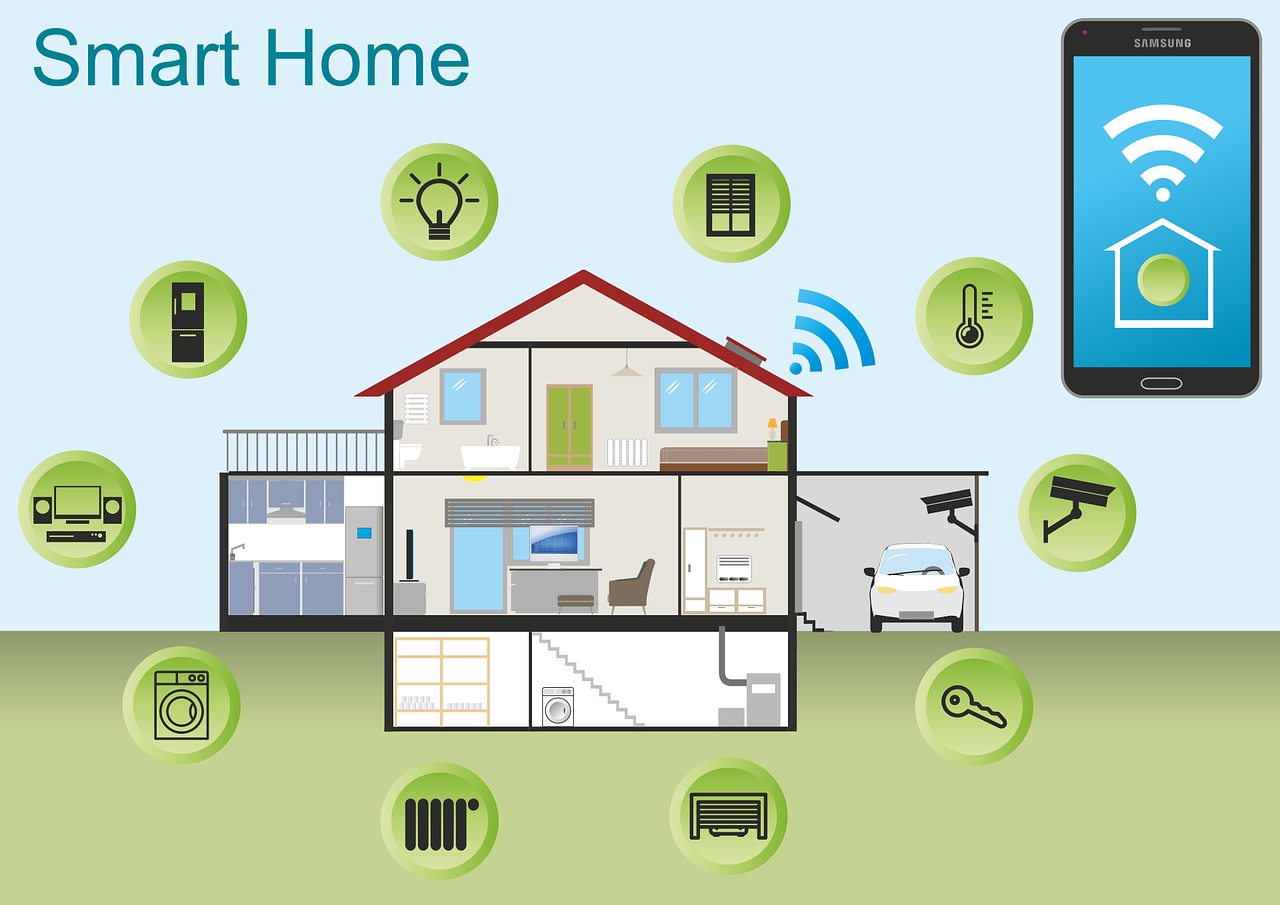
\includegraphics[scale=0.30]{resources/images/other/smart-home-example.png}
  \caption{
    L'idea di \textit{smart home}: tutti i dispositivi domestici sono connessi
    tra loro tramite Internet e possono essere controllati da remoto.
  }
  \label{fig:figure1.1}
\end{figure}

Normalmente, il controllo di questi dispositivi è affidato ad applicazioni
particolari, magari legate a uno specifico produttore. Queste prediligono un
setup facile e veloce, consentendo a chiunque di domotizzare la propria casa
senza troppe difficoltà e di controllarla generalmente tramite cellulare (ad
esempio, \textit{Philips Hue} \cite{PHILIPS}). Tuttavia, questi sistemi sono
spesso vincolati ai dispositivi di uno specifico produttore.

Quando alla \textit{smart home} si integrano dispositivi anche molto diversi
tra loro o addirittura incompatibili, diventa invece necessario un sistema di
controllo centralizzato. Solitamente, questi sistemi richiedono un setup
complesso e delle conoscenze abbastanza approfondite in materia, ma permettono
d'intermediare le interazioni tra i dispositivi, di controllarli molto più
liberamente e di creare delle regole di automazione più complesse (ad esempio,
\textit{OpenHAB} \cite{OPENHAB}).

Un altro dei vantaggi di una \textit{smart home} è la possibile integrazione
con un’assistente vocale: una tecnologia che consente d'interagire con il
proprio sistema domotico attraverso comandi vocali e di dare una voce ai propri
strumenti.

\subsection{Gli assistenti vocali}
\label{subsec:Sezione1.2.2}

Gli \textit{assistenti vocali} sono una tecnologia che si è diffusa
recentemente, il cui sviluppo risale tuttavia già al 1952, con il primo
dispositivo in grado di riconoscere delle cifre decimali in linguaggio parlato:
\textit{Audrey} di \textit{Bell Labs}. Dieci anni più tardi, fu \textit{IBM} a
proporre \textit{Shoebox}, il primo calcolatore in grado di riconoscere
operazioni matematiche in linguaggio parlato. Così, dagli anni '70 lo studio
degli assistenti vocali iniziò a diffondersi, fino a portare i risultati
odierni. \cite{VOCAL_ASSISTANT}

Oggi un’assistente vocale è uno strumento che permette d'interagire con dei
servizi attraverso dei comandi vocali. Nello specifico, è esso stesso un
servizio, basato sull’intelligenza artificiale e il \textit{machine learning},
capace di tradurre il linguaggio parlato in dati comprensibili a una macchina
(\textit{STT: Speech To Text}) e viceversa (\textit{TTS: Text To Speech}), così
proponendosi come ottimo intermediario nelle interazioni tra le persone e le
macchine.

Normalmente, si interagisce con un’assistente vocale tramite cellulare,
computer o tramite un apposito dispositivo del produttore specifico. Queste
però sono solo interfacce, infatti si occupano solo di registrare le richieste
dell’utente, per poi inviare le registrazioni al servizio vero e proprio per
essere interpretate. Tale servizio è solitamente installato su un
\textit{cloud}, ovvero su un insieme di cluster di macchine in remoto.

\begin{figure}[!ht]
  \centering
  \includegraphics[scale=0.19]{resources/images/other/alexa-and-google-assistant.png}
  \caption{
    Alcuni degli assistenti vocali più conosciuti insieme alla loro
    applicazione per cellulare: a sinistra, \textit{Alexa} di Amazon; a destra,
    \textit{Google Assistant} di Google.
  }
  \label{fig:figure1.2}
\end{figure}

Gli assistenti vocali possono essere utilizzati per agevolare l'accesso a
diversi servizi, ma spesso svolgono anche una funzione d'intrattenimento. Tra
le diverse funzionalità che offrono, esistono infatti dei giochi, basati
interamente su interazioni vocali. Prendendo ispirazione da ciò e seguendo i
principi di \textit{gamification}, si è deciso di sviluppare alcuni giochi per
un'assistente vocale, che avessero tuttavia anche un fine educativo,
specificamente il fine di esercitare alcune funzioni cognitive del cervello.

\subsection{Gamification e giochi cognitivi}
\label{subsec:Sezione1.2.3}

Con il termine \textit{gamification} s'intende \textit{"l'utilizzo di
meccanismi tipici del gioco e, in particolare, del videogioco (punti, livelli,
premi, beni virtuali, classifiche), per rendere gli utenti o i potenziali
clienti partecipi delle attività di un sito e interessarli ai servizi offerti"}
\cite{GAMIFICATION}. Nel dettaglio, i principi di gamification sono applicati a
un servizio quando si vuole:
\begin{itemize}
  \item[--] \textit{Aumentare la soddisfazione dell'utente}: la continua
        documentazione dei risultati del giocatore consente di visualizzare i
        propri progressi, facilitando la derivazione di obiettivi personali
        realizzabili e offrendo un feedback immediato sul comportamento
        dell'utente;
  \item[--] \textit{Trasmettere ottimismo all'utilizzatore}: la
        \textit{gamification} promuove l'autodeterminazione, oltre
        all'esperienza di un senso di realizzazione, o più specificamente la
        speranza di raggiungere gli obiettivi preposti;
  \item[--] \textit{Facilitare l'interazione sociale tra gli utilizzatori}:
        giocare significa spesso essere coinvolti in una comunità di giocatori,
        dando quindi spazio a scambi sociali e/o competizioni;
  \item[--] \textit{Motivare l'utente a utilizzare il servizio}: ciò assume
        particolare importanza se l'utente può realmente trarre vantaggio dal
        servizio (ad esempio, se il servizio ha uno scopo formativo)
        \cite{GAMIFICATION_PURPOSE}.
\end{itemize}

In questo elaborato, la \textit{gamification} viene applicata a un servizio che
permetterà l'accesso ad alcuni esercizi cognitivi. Ciò implica la progettazione
di \textit{giochi cognitivi}, ovvero di giochi che stimolano le funzioni
cognitive del cervello.

\subsection{Le funzioni cognitive del cervello}
\label{subsec:Sezione1.2.4}

Il cervello è uno degli organi più importanti e complessi del nostro corpo. La
sua complessità deriva dal fatto che ha la funzione di coordinare gran parte
dei meccanismi del nostro organismo, insieme alla percezione, il movimento, il
linguaggio, le emozioni e il pensiero.

Tra le funzioni del cervello vi sono quelle che prendono il nome di funzioni
cognitive. Le funzioni cognitive sono processi mentali che consentono
d'interagire con il mondo esterno e processare gli stimoli ricevuti producendo
pensieri complessi. Esse si distinguono in alcune macro-categorie:
\begin{itemize}
  \item \textbf{Attenzione}: è un insieme di processi complessi che
        permettono di selezionare alcuni stimoli specifici tra tutti quelli
        provenienti dall’ambiente circostante. Esistono diversi livelli di
        attenzione, organizzati su una struttura piramidale, per cui
        l’attivazione di un livello richiede quella di tutti i livelli
        sottostanti. I livelli di attenzione sono, dalla base alla cima della
        piramide:
        \begin{itemize}
          \item[o] \textbf{Attenzione sostenuta}: è la capacità di mantenere
                l’attenzione nel tempo, reagendo agli stimoli provenienti
                dall'ambiente circostante, anche detta concentrazione o
                vigilanza;
          \item[o] \textbf{Attenzione selettiva}: è la capacità di rimanere
                concentrati su uno specifico compito, inibendo gli altri
                stimoli esterni (come il rumore di sottofondo);
          \item[o] \textbf{Attenzione alternata}: è la capacità di eseguire più
                compiti, concentrandosi su un compito per volta in modo
                alternato;
          \item[o] \textbf{Attenzione divisa}: è la capacità di rimanere
                concentrati su più compiti contemporaneamente.
        \end{itemize}
  \item \textbf{Memoria}: è il processo che permette la codifica degli
        stimoli esterni, in modo da essere memorizzati e quindi recuperabili in
        un secondo momento. La memoria è applicata ai soli eventi a cui si è
        prestata attenzione. In particolare, si distinguono:
        \begin{itemize}
          \item[o] \textbf{Memoria a lungo termine}: è la memoria riservata a
                enormi quantità d'informazioni per un periodo di tempo molto
                lungo;
          \item[o] \textbf{Memoria a breve termine}: è la memoria riservata a
                piccole quantità d'informazioni per una durata di al massimo 30
                secondi circa; queste informazioni possono essere rielaborate
                per passare alla memoria a lungo termine, altrimenti sono
                perse.
        \end{itemize}
  \item \textbf{Orientamento}: è la capacità di riconoscere e comprendere ciò
        che dovrebbe esserci familiare. Comprende sia l’orientamento spaziale,
        ma anche il riconoscimento dei volti e degli oggetti.
  \item \textbf{Linguaggio}: è la capacità di esprimere o comprendere dei
        pensieri attraverso dei simboli, che spesso si manifestano come lingue.
        Alcune funzioni del linguaggio sono:
        \begin{itemize}
          \item[o] \textbf{Semantica}: la capacità di distinguere parole che
                hanno significati, tali da essere accomunabili sotto a una
                stessa categoria;
          \item[o] \textbf{Fonemica}: la capacità di distinguere parole che
                hanno un suono simile.
        \end{itemize}
  \item \textbf{Funzioni esecutive}: sono l’insieme di tutte le funzioni
        cognitive superiori, che includono il controllo della cognizione e la
        regolazione dei pensieri, come ad esempio l’astrazione, la deduzione e
        la pianificazione.
\end{itemize}

Con l’invecchiamento, si assiste a un decremento delle prestazioni cognitive,
soprattutto per le abilità cognitive soggette a disuso o poco stimolate. Questo
può prevedere:
\begin{itemize}
  \item[--] Un \textit{rallentamento dei tempi di reazione}, prolungando il
        tempo impiegato a svolgere determinati compiti;
  \item[--] Un \textit{deficit dell’attenzione}, che è in realtà la causa di
        molti dei problemi di memoria accusati dagli anziani;
  \item[--] Un \textit{deficit delle funzioni esecutive}, che può ad esempio
        rendere più difficile monitorare processi complessi o inibire certi
        comportamenti inadeguati;
  \item[--] Un \textit{deficit della memoria}, soprattutto
        \textit{a breve termine}, mentre quella a lungo termine è meno affetta.
\end{itemize}

Per contrastare queste conseguenze, in generale, è sufficiente cercare di
mantenere uno stile di vita sano, in termini di socialità, dieta, esercizio
fisico e attività mentale. Un’altra ricetta anti-invecchiamento è invece
l’impostazione di abitudini costruttive, perché per imparare a fare una cosa,
come per ricordarsela, bisogna continuare a farla nel tempo. \cite{SOM}
% ! TeX root = ../bachelor-thesis.tex

\chapter{Studio del problema}
\label{ch:Chapter2}

In questo capitolo si analizzerà la natura del problema che si vuole risolvere,
identificando i requisiti che il sistema dovrà soddisfare per adempiere al suo
scopo.

Nello specifico, si formalizzeranno le funzioni che il sistema deve poter
assolvere, classificandole in base alla loro priorità. Inoltre, si discuteranno
quei vincoli del sistema che dipendono dalla sua stessa natura.

\section{Analisi dei requisiti}
\label{sec:Sezione2.1}

Ora si descriveranno in un modo più ordinato e formale i requisiti del sistema
da progettare.

Più in dettaglio, i requisiti saranno categorizzati attraverso la
prioritizzazione MoSCoW \cite{MOSCOW}. Si distingueranno quindi i requisiti
\textit{must have}, ovvero quelli vitali, che devono essere soddisfatti dal
sistema a breve termine, i requisiti \textit{should have}, ovvero quelli
importanti, che dovranno essere soddisfatti dal sistema a lungo termine, e i
requisiti \textit{could have}, ovvero quelli opzionali, che potranno essere
integrati una volta ultimato il sistema. In questa tesi progettuale, lo scopo
preposto è quello di soddisfare almeno i requisiti \textit{must have}, quindi
tutti gli schemi trattati, faranno riferimento esclusivamente a quei requisiti.

\subsection{Must Have}
\label{subsec:Sezione2.1.1}

Il sistema dovrà assolutamente soddisfare i seguenti requisiti funzionali:

\begin{enumerate}
  \item[\textbf{A.}] \textit{\textbf{Controllo dei dispositivi domotici da
            sistema di controllo.}} Sarà necessario fornire all’utente un
        sistema di controllo, attraverso il quale si potrà interagire per
        monitorare e controllare i propri dispositivi domotici.
  \item[\textbf{B.}] \textit{\textbf{Controllo dei dispositivi domotici
            attraverso comandi vocali.}} Sarà necessario fornire all’utente
        un’assistente vocale, integrato con il sistema di controllo domotico,
        attraverso il quale si potrà controllare i propri dispositivi domotici
        attraverso comandi vocali.
  \item[\textbf{C.}] \textit{\textbf{Ricezione delle notifiche dai dispositivi
            domotici.}} Sarà necessario fornire all’utente la possibilità di
        ricevere delle notifiche sugli eventi rilevati dai dispositivi
        domotici, sia tramite il sistema di controllo domotico, sia tramite
        l’assistente vocale (quando più opportuno).
  \item[\textbf{D.}] \textit{\textbf{Accesso allo storico degli eventi rilevati
            dai dispositivi domotici.}} Sarà necessario registrare tutti gli
        eventi rilevati dai dispositivi domotici fino a un certo periodo di
        tempo, così da fornire all’utente la possibilità di consultare lo
        storico degli eventi tramite il sistema di controllo domotico.
  \item[\textbf{E.}] \textit{\textbf{Accesso ad almeno tre giochi cognitivi
            distinti tramite l’assistente vocale.}} Sarà necessario fornire
        all’utente un servizio comprendente almeno tre giochi cognitivi tra
        cui poter scegliere e a cui poter accedere attraverso l’assistente
        vocale. I giochi cognitivi dovranno distinguersi in base alle
        capacità cognitive di cui permetteranno l’allenamento.
\end{enumerate}

Di seguito, il diagramma dei casi d’uso che schematizza questi specifici
requisiti, che saranno quelli trattati successivamente nella tesi (Figura
\ref{fig:figure2.1}).

\begin{figure}[H]
  \centering
  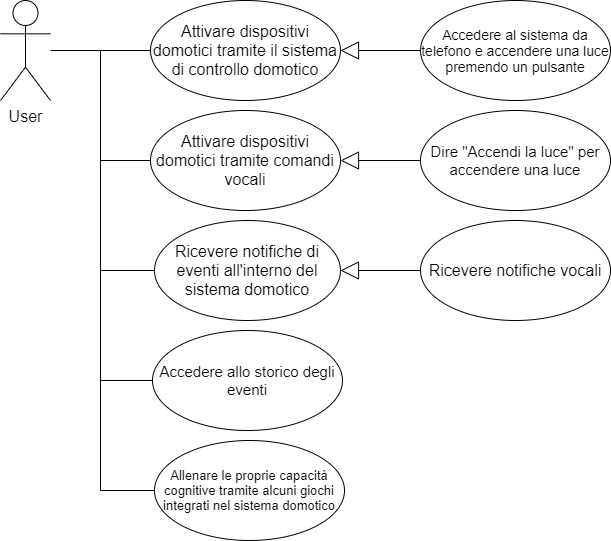
\includegraphics[scale=0.5]{resources/images/analysis/use-cases-diagram.jpg}
  \caption{
    Il diagramma dei casi d'uso che riassume i requisiti funzionali del
    sistema.
  }
  \label{fig:figure2.1}
\end{figure}

\subsection{Should Have}
\label{subsec:Sezione2.1.2}

In un secondo momento, il sistema dovrà evolversi soddisfacendo i seguenti
requisiti funzionali:

\begin{enumerate}
  \item[\textbf{F.}] \textit{\textbf{Gestione dell’autenticazione come paziente
            o personale socio-sanitario.}} Sarà necessario gestire
        l’autenticazione, introducendo delle credenziali per essere
        riconosciuti come pazienti o come personale socio-sanitario.
  \item[\textbf{G.}] \textit{\textbf{Accesso allo storico dei risultati
            ottenuti sui diversi giochi cognitivi di un determinato paziente.}}
        Sarà necessario registrare il risultato ottenuto dal paziente alla fine
        di ciascuna partita, per ogni gioco cognitivo, così da fornire un
        campione di dati analizzabile per monitorare e comprendere i
        miglioramenti conseguiti dal paziente. Questo storico sarà accessibile
        solo a personale socio-sanitario autorizzato.
  \item[\textbf{H.}] \textit{\textbf{Analisi dei risultati ottenuti sui diversi
            giochi cognitivi.}} Sarà necessario implementare un servizio,
        possibilmente scalabile, che potrà accedere ai risultati ottenuti
        da uno specifico paziente, così da poter eseguire un’analisi più
        dettagliata dei risultati del paziente e produrre un report dei
        progressi, visualizzabile dal personale socio-sanitario
        autorizzato.
  \item[\textbf{I.}] \textit{\textbf{Gestione del percorso educativo di un
            paziente.}} Sarà necessario permettere al personale socio-sanitario
        autorizzato d'impostare un percorso educativo per un dato
        paziente, che preveda una routine di giochi cognitivi, da proporre
        a tale paziente attraverso l’assistente vocale.
  \item[\textbf{J.}] \textit{\textbf{Aggiunta di nuovi giochi cognitivi.}}
        Sarà necessario espandere il servizio che fornisce i giochi cognitivi,
        in modo da coprire più capacità cognitive, ma anche fornire più varietà
        per allenare la stessa capacità cognitiva.
\end{enumerate}

\subsection{Could Have}
\label{subsec:Sezione2.1.3}

Di seguito, i requisiti considerati opzionali, ovvero che potrebbero essere
implementati nei tempi successivi al completamento del sistema:

\begin{enumerate}
  \item[\textbf{K.}] \textit{\textbf{Accesso ai giochi cognitivi al di fuori
            del contesto socio-sanitario.}} Sarà opzionale consentire l’accesso
        ai giochi cognitivi al di fuori del contesto socio-sanita\-rio, così
        da poterli installare su altri sistemi domotici pubblici o privati.
  \item[\textbf{L.}] \textit{\textbf{Suggerimento casuale di un gioco
            cognitivo.}} Sarà opzionale permettere all’assistente vocale di
        proporre all’utente uno dei giochi cognitivi installati, a discrezione
        dell’utente.
  \item[\textbf{M.}] \textit{\textbf{Ulteriore aggiunta di nuovi giochi
            cognitivi.}} Sarà opzionale espandere nuovamente il servizio che
        fornisce i giochi cognitivi, in modo da coprire più capacità cognitive,
        ma anche fornire più varietà per allenare la stessa capacità cognitiva.
\end{enumerate}

\section{Vincoli del Sistema}
\label{sec:Sezione2.2}

Ora si illustreranno alcuni dei vincoli del sistema, dovuti alla natura del
sistema stesso.

Il primo vincolo è dovuto ai \textbf{costi}. Infatti configurare un sistema
domotico, che sia un impianto o una \textit{smart home} (o entrambi), ha dei
costi non irrisori per l’acquisto dei dispositivi, soprattutto se si tratta di
dispositivi progettati per l’accessibilità.

Il secondo vincolo è dovuto all’uso di un assistente vocale. Gli assistenti
vocali si basano su \textit{cloud computing}, che ha enormi vantaggi in termini
di fruibilità di risorse e scalabilità, tuttavia ha anche qualche svantaggio.

In primo luogo, gli assistenti vocali necessitano di una connessione a
Internet, anzi più specificamente necessitano di una \textbf{connessione verso
il cloud del produttore}. In altre parole, se, per un qualche motivo, un giorno
non è possibile raggiungere il cloud del produttore, quel giorno l’assistente
vocale non potrà funzionare (perciò non si potrà accedere ai giochi cognitivi,
né utilizzarlo per controllare il proprio sistema domotico).

In secondo luogo, vi è la questione della \textbf{privacy} e della
\textbf{sicurezza}. Infatti, gli assistenti vocali inviano le registrazioni
vocali al cloud del produttore per essere processate e dunque interpretate come
linguaggio parlato. Questo chiaramente richiede un alto livello di fiducia da
parte dell’utilizzatore. Risulta quindi necessaria un’infrastruttura di rete
sicura e un rispetto adeguato delle norme di privacy e sicurezza da parte dei
produttori.

Fortunatamente, molti produttori hanno recentemente adottato un’infrastruttura
che promuova l’\textit{edge computing}, ovvero una forma di cloud computing,
che sposta i centri di calcolo verso gli utilizzatori, riducendo il tempo per
cui i loro dati si trovano in rete e migliorando anche la responsività e
fruibilità dei servizi forniti, tra cui gli assistenti vocali.

Un terzo e ultimo vincolo è infine dovuto alla natura dei giochi, che si basano
strettamente su interazioni vocali. Ciò rende \textbf{difficile realizzare
giochi troppo complessi}, in cui la quantità d'informazioni da scambiare è
molto elevata. In questi giochi, infatti, risulterebbe più efficace una
comunicazione parallela, basata su più sensi (come vista e udito), piuttosto
che una seriale, come un’interazione vocale, che si basa solo sull’udito. Per
fortuna però, molti esercizi cognitivi si basano su interazioni semplici e si
prestano piuttosto bene a essere implementati attraverso un’assistente vocale.

% ! TeX root = ../bachelor-thesis.tex

\chapter{Progettazione del sistema}
\label{ch:Chapter3}

In questo capitolo si proporrà una possibile soluzione che soddisfa i requisiti
\textit{must have} del sistema descritto precedentemente.

Più in dettaglio, si analizzeranno le tecnologie scelte per implementare il
sistema, focalizzandosi prima sul loro funzionamento individuale e
successivamente su come possono interagire tra di loro. Inoltre, sarà
giustificata la scelta di tali tecnologie nel contesto in cui è stato
sviluppato il progetto. Infine, si illustreranno alcune possibili limitazioni
del sistema, non più dipendenti dalla natura del problema stesso, ma derivanti
dalle tecnologie specifiche utilizzate per implementarlo.

\section{Architettura del Sistema}
\label{sec:Sezione3.1}

Ora si descriverà una possibile soluzione al problema introdotto nei capitoli
precedenti, facendo riferimento ai requisiti \textit{must have} del sistema.

In particolare, si progetterà prima un’architettura di massima che descriva
quali sono i componenti e le interazioni che appartengono al sistema, dopodiché
s’illustrerà l’architettura effettivamente implementata, vincolata alle
specifiche tecnologie scelte.

\subsection{Architettura di massima}
\label{subsec:Sezione3.1.1}

Di seguito, viene proposta un’architettura generica di massima che possa
soddisfare i requisiti \textit{must have} del problema (Figura
\ref{fig:figure3.1}).

\begin{figure}[!ht]
  \centering
  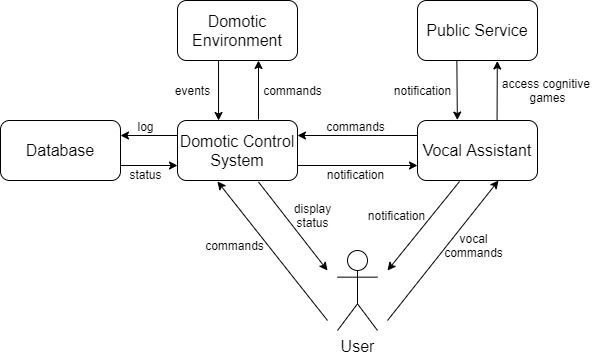
\includegraphics[scale=0.7]{resources/images/design/system-structure-analysis-diagram.jpg}
  \caption{Lo schema delle interazioni in una generalizzazione del sistema.}
  \label{fig:figure3.1}
\end{figure}

L’\textbf{utente} potrà interfacciarsi con il sistema attraverso il
\textbf{sistema di controllo domotico} e l’\textbf{assistente vocale}. Entrambi
gli permetteranno di controllare il proprio \textbf{ambiente domotico},
composto da tutti i dispositivi domotici del sistema. Il sistema di controllo
domotico registrerà anche gli eventi ricevuti dall’ambiente domotico in un
\textbf{database} e consentirà all’utente di accedere allo stato corrente e
allo storico degli stati dei suoi dispositivi domotici. Inoltre, potrà
notificare l’utente di certi eventi accaduti, attraverso messaggi vocali
mediati dall’assistente vocale. L’assistente vocale, oltre a delegare i comandi
vocali rivolti verso l’ambiente domotico al sistema di controllo domotico,
permetterà l’accesso agli esercizi cognitivi. Questi saranno esposti attraverso
un \textbf{servizio pubblico}, quindi accessibile dall’assistente vocale.

\subsection{Progetto del sistema}
\label{subsec:Sezione3.1.2}

Dopo aver descritto l’architettura di massima, ora si riporterà un’architettura
vincolata alle tecnologie scelte per implementare il sistema (Figura
\ref{fig:figure3.2}).

\begin{figure}[!ht]
  \centering
  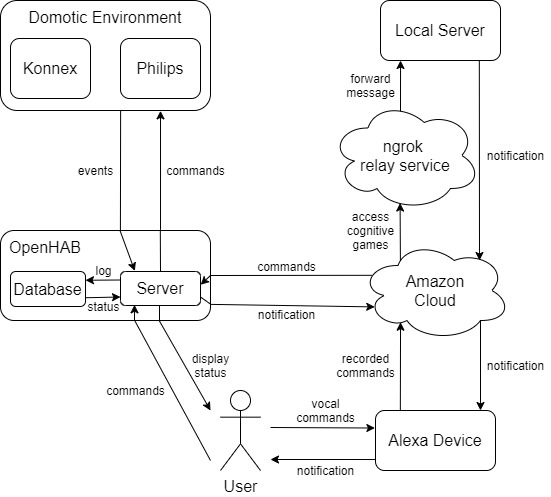
\includegraphics[scale=0.6]{resources/images/design/system-structure-design-diagram.jpg}
  \caption{
    Lo schema delle interazioni nel sistema che sarà implementato in questo
    elaborato.
  }
  \label{fig:figure3.2}
\end{figure}

Più in dettaglio, le tecnologie scelte sono:
\begin{itemize}
  \item[--] Per l’\textit{ambiente domotico}, si è scelta una smart home
        composta da un impianto domotico \textbf{KNX} \cite{KONNEX} e alcuni
        dispositivi smart della \textbf{Philips} \cite{PHILIPS}. Questo
        sistema era già predisposto su di un appartamento usato come caso di
        studio;
  \item[--] Per il \textit{sistema di controllo domotico}, è stato scelto
        \textbf{OpenHAB} \cite{OPENHAB}, perché consente di gestire una grande
        varietà di dispositivi domotici e quindi di non vincolarsi a uno
        specifico produttore. In aggiunta, è anche comprensivo di un database.
        Questo sistema era in gran parte già predisposto per controllare
        l’appartamento domotico;
  \item[--] Per l’\textit{assistente vocale}, è stata scelta \textbf{Amazon
          Alexa} \cite{ALEXA}, nello specifico un dispositivo
        \textit{\textbf{Alexa Echo Dot}}, poiché già disponibile da ricerche
        e studi precedenti;
  \item[--] Per gli \textit{esercizi cognitivi}, allo scopo di eliminare i
        costi di manutenzione di un server pubblico, è stato scelto
        d'implementare un servizio su un server locale, esposto come server
        pubblico tramite \textbf{ngrok} \cite{NGROK}, ovvero un servizio
        gratuito in cloud che inoltra le richieste ricevute a una specifica
        porta di una macchina locale.
\end{itemize}

\section{Tecnologie utilizzate}
\label{sec:Sezione3.2}

In questo capitolo, si entrerà più nel dettaglio rispetto alle tecnologie
utilizzate nel progetto, spiegando come vengono realizzate le interazioni tra i
vari componenti del sistema.

Dunque, saranno prima descritte le caratteristiche di OpenHAB, come sistema di
controllo domotico, poi di Alexa, come assistente vocale, e infine saranno
descritti i servizi che offrono per interfacciarsi l’uno con l’altro.

\subsection{OpenHAB come sistema di controllo domotico}
\label{subsec:Sezione3.2.1}

\textbf{OpenHAB} (Open Home Automation Bus) è una piattaforma che gestisce la
comunicazione e l’automazione in un ambiente domotico, svincolandosi dalle
specifiche tecnologie utilizzate dai dispositivi che controlla. Le sue
caratteristiche principali sono:
\begin{itemize}
  \item[--] La possibilità d'\textit{integrare dispositivi domotici anche
          molto diversi}, permettendo loro di comunicare indirettamente,
        persino se usano tecnologie e/o protocolli direttamente
        incompatibili;
  \item[--] La possibilità di controllare il proprio ambiente domotico
        attraverso un’\textit{unica interfaccia utente} e di creare
        \textit{regole di automazione per la casa uniche e valide su tutto il
          sistema}, evitando di utilizzare un’applicazione diversa per ogni
        specifico produttore;
  \item[--] È un software \textit{open source}, quindi, oltre a essere
        gratuito, possiede una comunità di sviluppatori che estendono
        continuamente le sue funzionalità. \cite{OPENHAB_DOC}
\end{itemize}

\subsubsection{3.2.1.1. La comunicazione con i dispositivi domotici}
\label{subsec:Sezione3.2.1.1}

La struttura con cui OpenHAB consente l’interazione con i dispositivi connessi,
si basa su diversi livelli d'interfacciamento (come descritto in Figura
\ref{fig:figure3.3}).

\begin{figure}[!ht]
  \centering
  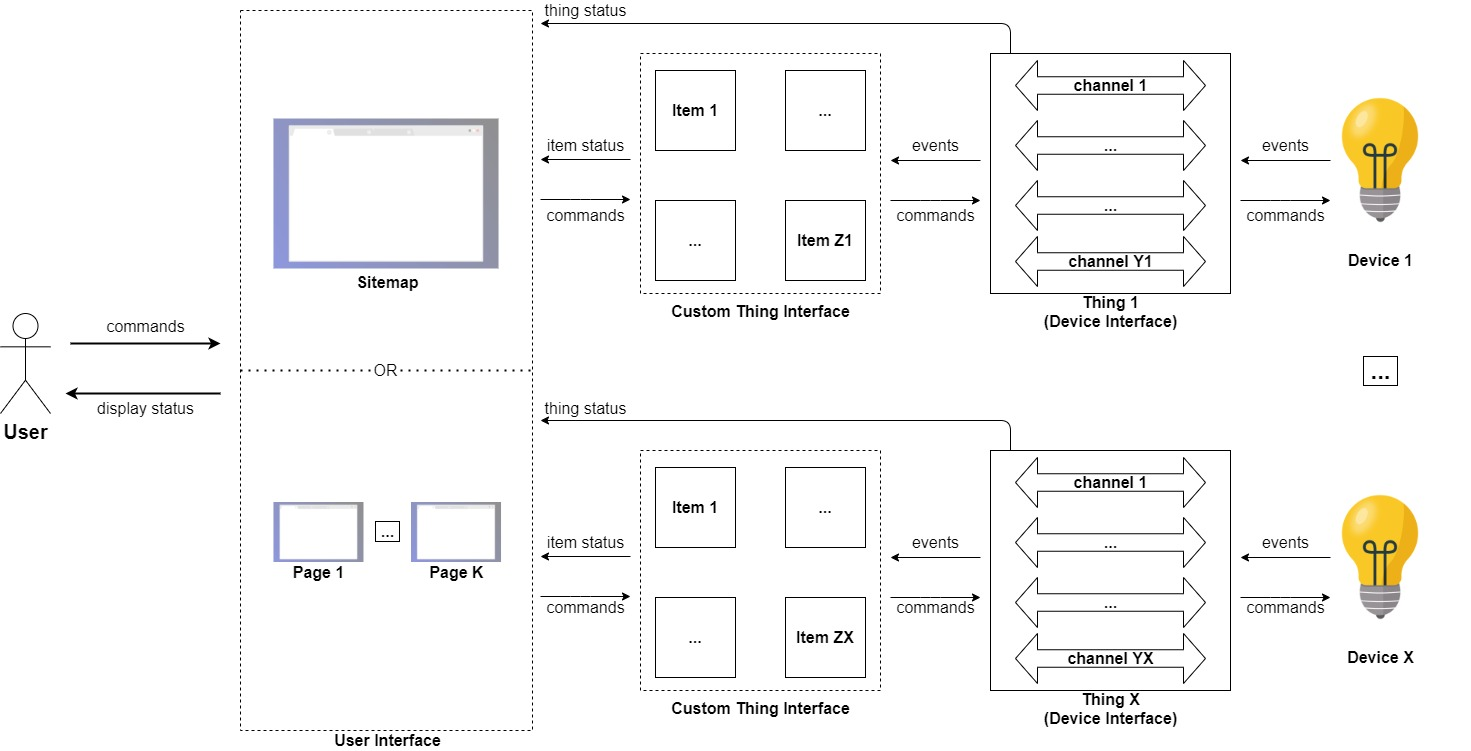
\includegraphics[scale=0.3]{resources/images/other/openhab-control-flow.jpg}
  \caption{
    I diversi livelli d'interfacce poste tra l'utente e i suoi dispositivi
    domotici in OpenHAB.
  }
  \label{fig:figure3.3}
\end{figure}

Il primo livello d'interfacciamento è costituito dalle \textit{\textbf{things}}
\cite{THINGS}, che espongono le funzionalità di un dispositivo fisico
all’interno di OpenHAB, attraverso i \textit{\textbf{channel}} di cui sono
composte. Ciascun \textit{channel} espone una specifica funzione del
dispositivo domotico. Ogni \textit{thing} mantiene lo stato della connessione
tra il dispositivo fisico che controlla e OpenHAB, ad esempio se il dispositivo
è raggiungibile (\textit{ONLINE}) o meno (\textit{OFFLINE}).

Il secondo livello d'interfacciamento è costituito dagli
\textit{\textbf{items}} \cite{ITEMS}. Esistono diversi tipi di \textit{item},
ognuno dei quali si distingue per gli stati che può assumere e i comandi che
può ricevere. Un \textit{item} può essere associato a più \textit{channel}, che
controllerà inoltrando loro i comandi che riceve. Viceversa, un
\textit{channel} può essere associato a più \textit{item}, da cui sarà
controllato. Gli \textit{item} offrono un certo grado di libertà e permettono
di scegliere con quali comandi si vuole controllare i propri dispositivi, al
contrario delle \textit{thing}, che sono spesso vincolate dal dispositivo
fisico che rappresentano.

L’ultimo livello d'interfacciamento è costituito dall'\textbf{interfaccia
utente}, esposta attraverso il \textit{Web Server di OpenHAB} e quindi
accessibile tramite browser. All’interno di OpenHAB ne esistono di diversi
tipi, ma le più recenti sono:
\begin{itemize}
  \item \textit{\textbf{Sitemap}} \cite{SITEMAP}: un’interfaccia dalla grafica
        minimale e funzionale;
  \item \textit{\textbf{Pages}} \cite{PAGES}: un’interfaccia dalla grafica più
        accattivante e user-friendly.
\end{itemize}
Le componenti grafiche con cui si controlla un \textit{item} dall’interfaccia
utente sono determinate dal tipo di quell’\textit{item}.

Di seguito, si riporta un esempio che integra quanto detto finora (Figura
\ref{fig:figure3.4}).
\begin{figure}[!ht]
  \centering
  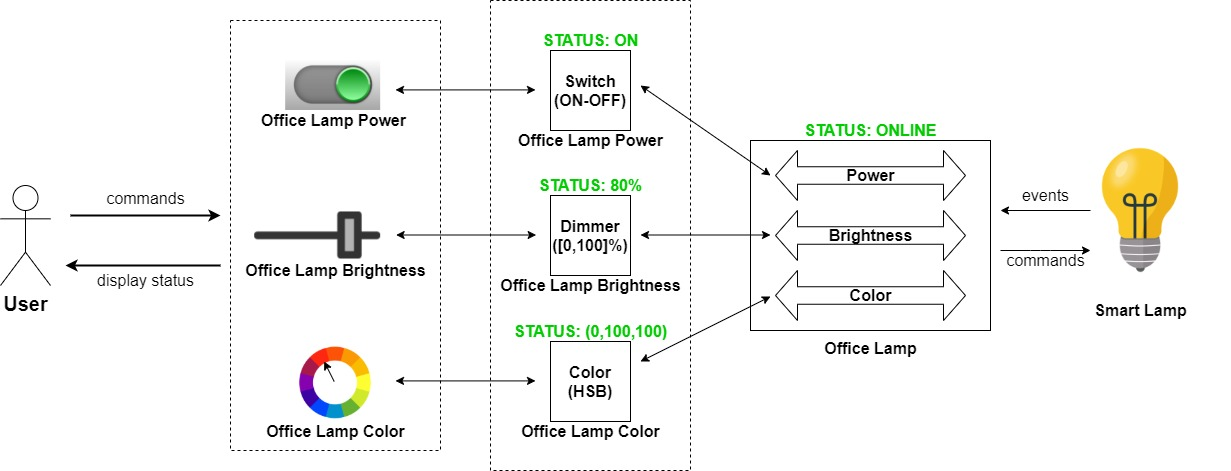
\includegraphics[scale=0.36]{resources/images/other/openhab-lamp-example.jpg}
  \caption{
    Esempio d'interfacciamento tra l'utente e una lampadina smart tramite
    OpenHAB.
  }
  \label{fig:figure3.4}
\end{figure}

\subsubsection{3.2.1.2. Add-On, Automazione e Persistenza}
\label{subsec:Sezione3.2.1.2}

Alle componenti principali, che permettono la comunicazione tra OpenHAB e i
dispositivi domotici, si aggiungono delle componenti più avanzate.

In primo luogo, i \textit{\textbf{binding}} \cite{BINDING} sono degli
\textit{add-on} che aggiungono ulteriori funzionalità a OpenHAB. Normalmente, i
\textit{binding} forniscono nuove tipologie di \textit{thing}, che possiedono
\textit{channel} preconfigurati per connettere a OpenHAB dispositivi di una
certa categoria. Ad esempio, esistono \textit{binding} per dispositivi domotici
di diversi produttori (come \textit{Philips Hue Binding}).

In secondo luogo, le \textit{\textbf{rule}} \cite{RULES} gestiscono la parte di
automazione di OpenHAB. In particolare, sono degli \textit{handler} che possono
accedere e inviare comandi agli \textit{item} in risposta a particolari eventi.

Infine, la \textit{\textbf{persistence}} \cite{PERSISTENCE} consente di
costruire uno storico degli stati e degli eventi ricevuti, memorizzandoli sul
database integrato di OpenHAB. È infatti possibile configurare OpenHAB in modo
che campioni automaticamente lo stato di alcuni \textit{item} indicati. Il
metodo di campionamento può essere descritto attraverso una
\textit{\textbf{strategy}}, che indica ogni quanto e sotto quali condizioni
campionare gli \textit{item}.

\subsection{Alexa come assistente vocale}
\label{subsec:Sezione3.2.2}

\textbf{Amazon Alexa} \cite{ALEXA}, o semplicemente Alexa, è un’assistente
vocale sviluppato da Amazon. Più precisamente, è un servizio del cloud di
Amazon capace d'interpretare la voce umana producendo del testo, e viceversa,
dunque permettendo un’interazione vocale con altri servizi, sotto la sua
mediazione.

Le applicazioni di Alexa sono numerose, ma principalmente includono:
\begin{itemize}
  \item[--] Lo \textit{sviluppo di Alexa Skills}, ovvero di servizi pubblici
        accessibili tramite comandi vocali;
  \item[--] Lo \textit{sviluppo di dispositivi Alexa-Integrated}, ovvero di
        strumenti controllabili attraverso comandi vocali;
  \item[--] L’agevolazione del monitoraggio e della gestione degli ambienti di
        lavoro tramite \textit{Alexa for Business}.
\end{itemize}
In questo progetto, Alexa sarà utilizzata per interagire, oltre che con il
sistema domotico, anche con gli esercizi cognitivi, che saranno quindi
implementati come \textit{\textbf{skills}} di Alexa.

\subsubsection{3.2.2.1. Alexa Skill}
\label{subsec:Sezione3.2.2.1}

Una \textit{skill} di Alexa è composta principalmente da:
\begin{itemize}
  \item[--] Un \textbf{nome d’invocazione}, che la identifica ed è utilizzato
        per accedere alla \textit{skill};
  \item[--] Un \textbf{modello di dialogo}, situato all’interno del cloud di
        Alexa, che indica le intenzioni che l’utente può esprimere
        all’assistente vocale all’interno della \textit{skill};
  \item[--] Un \textbf{modello logico}, situato nell’endpoint specificato, che
        indica quali saranno le reazioni della \textit{skill} in relazione alle
        intenzioni espresse dall’utente;
  \item[--] Un \textit{\textbf{endpoint}}, ovvero un indirizzo URL verso il
        servizio che implementa il modello logico della \textit{skill}.
\end{itemize}

Per interagire con una certa \textit{skill} è necessario richiamare il suo nome
d'invocazione all’interno dei comandi vocali espressi. In alternativa, è
possibile aprirla come un’applicazione qualsiasi (ad esempio, dicendo
\textit{"Alexa, apri Corriere della Sera."}). In tal caso, Alexa si aspetterà
solo comandi compresi nel modello di dialogo di quella \textit{skill}.

L’interazione con una \textit{skill} di Alexa avviene come mostrato in Figura
\ref{fig:figure3.5}.

\begin{figure}[!ht]
  \centering
  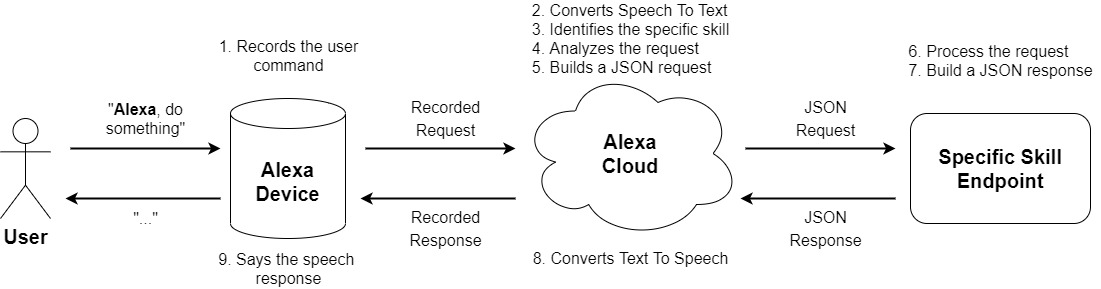
\includegraphics[scale=0.35]{resources/images/other/alexa-skill-flow.jpg}
  \caption{
    Il flusso d'interazione tra l'utente e una \textit{skill} di Alexa che
    permette d'innescare la reazione di un sistema tramite comandi vocali.
  }
  \label{fig:figure3.5}
\end{figure}

Inizialmente, l’utente esprime la propria intenzione a un \textbf{dispositivo
Alexa}, ad esempio un \textit{Alexa Echo Dot}. Per farlo, dovrà precedere il
comando vocale da una \textit{\textbf{wake-word}} (di default
\textit{“Alexa”}), ovvero una parola che indicherà al dispositivo di cominciare
a registrare. Una volta terminata la registrazione del comando vocale, il
dispositivo la inoltrerà al \textbf{cloud di Alexa}, per essere interpretata.
Giunta al cloud di Alexa, la registrazione sarà convertita in un comando
testuale, che sarà analizzato per identificare la \textit{skill} a cui si
riferisce e l’intenzione espressa dall’utente all’interno di quella
\textit{skill}. Il cloud inoltrerà quindi i risultati dell’analisi
all’\textit{\textbf{endpoint}} della \textit{skill} specifica. Ricevuta
l’intenzione dell’utente, l’\textit{endpoint} potrà reagire di conseguenza e
produrre una risposta testuale, che sarà successivamente tradotta dal cloud di
Alexa in una risposta vocale e infine comunicata dal dispositivo Alexa.

Come \textit{endpoint} dove collocare la logica della \textit{skill}, è
possibile scegliere tra diverse soluzioni, come mostrato in Figura
\ref{fig:figure3.6}, ognuna con i propri vantaggi e svantaggi:
\begin{itemize}
  \item[--] \textit{\textbf{Amazon Web Services (AWS) Lambda}}
        \cite{AWS_LAMBDA}: è un servizio in cloud di Amazon che permette di
        eseguire il proprio codice senza dover configurare e mantenere un
        proprio server; è scalabile e facile da usare, tuttavia ha un costo
        mensile basato sul numero di richieste ricevute e sulle risorse
        utilizzate;
  \item[--] Un \textit{\textbf{proprio cloud}}, ovvero un gruppo di cluster di
        macchine gestito in proprio; è scalabile e completamente
        personalizzabile, tuttavia ha una configurazione relativamente più
        lunga e un costo di gestione elevato;
  \item[--] Un \textit{\textbf{proprio server pubblico}}, ovvero una macchina
        accessibile da Internet; è la soluzione meno costosa ed è completamente
        personalizzabile, tuttavia ha una configurazione relativamente più
        lunga e soprattutto non è scalabile, che per un servizio accessibile
        pubblicamente è un grande svantaggio.
\end{itemize}

\begin{figure}[!ht]
  \centering
  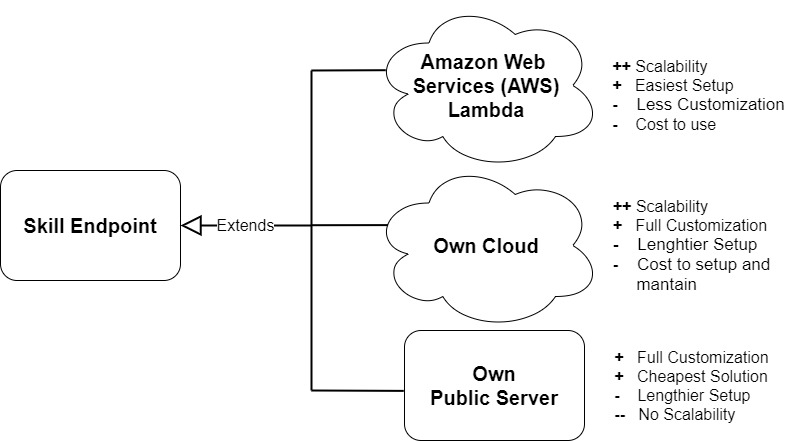
\includegraphics[scale=0.42]{resources/images/other/skill-endpoint-solutions.jpg}
  \caption{
    Le possibili soluzioni adottabili per implementare una \textit{skill} di
    Alexa.
  }
  \label{fig:figure3.6}
\end{figure}

Per minimizzare i costi di progettazione, si è scelta una soluzione a costo
zero, basata su un server locale esposto come server pubblico attraverso il
servizio gratuito \textit{ngrok}.

È possibile sviluppare una nuova \textit{skill} per Alexa interamente
attraverso l’\textbf{Amazon Developer Console} \cite{AMAZON_DEVELOPER_CONSOLE}:
una piattaforma online, gestita da Amazon, che permette l’accesso a diversi
strumenti di sviluppo software. In particolare, per lo sviluppo di una
\textit{skill} esiste uno strumento chiamato \textbf{ASK} (Alexa Skills Kit)
\cite{ASK}.

\subsubsection{3.2.2.2. Il modello di dialogo di una Alexa Skill}
\label{subsec:Sezione3.2.2.2}

Il modello di dialogo di una \textit{skill} di Alexa definisce le intenzioni
(\textit{\textbf{intents}}) che l’utente può esprimere all’interno della
\textit{skill}. Ogni \textit{intent} è associato a una serie di proposizioni
(\textit{\textbf{utterances}}), che l’utente può pronunciare per esprimere
quell’intenzione.

Un \textit{utterance} può contenere degli \textit{\textbf{slot}}, ovvero degli
spazi all’interno della proposizione, identificati da un nome, che possono
assumere un certo dominio di valori, definito dal \textbf{tipo di slot}.

Esistono due categorie a cui può appartenere un tipo di slot:
\begin{itemize}
  \item[--] \textit{Custom slot type}: è un tipo di slot il cui dominio di
        valori è un insieme finito definito dallo sviluppatore della
        \textit{skill};
  \item[--] \textit{Pre-built slot type}: è un tipo di slot il cui dominio di
        valori è predisposto da Amazon.
\end{itemize}

Di seguito, viene riportato uno schema che riassume i componenti appena
descritti (Figura \ref{fig:figure3.7}).
\begin{figure}[!ht]
  \centering
  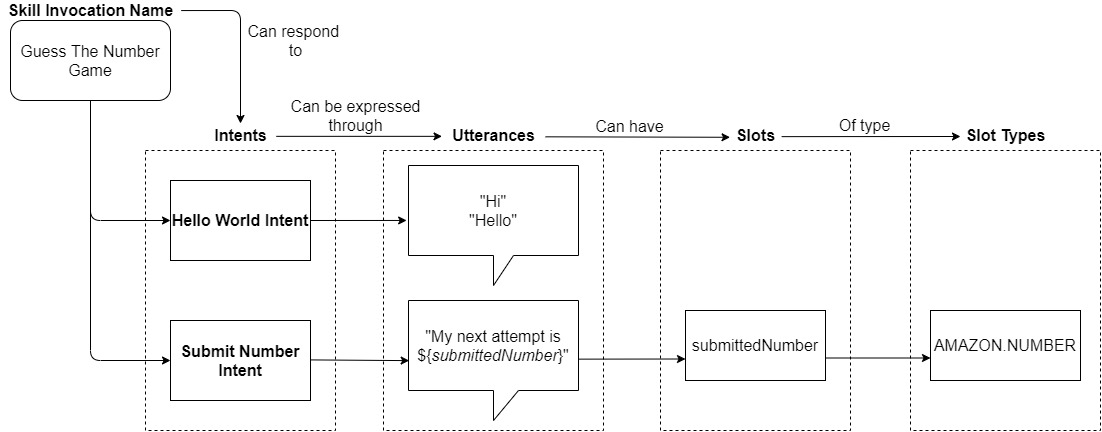
\includegraphics[scale=0.41]{resources/images/other/alexa-skill-dialog-model.jpg}
  \caption{Le componenti del modello di dialogo di una \textit{skill} di Alexa.}
  \label{fig:figure3.7}
\end{figure}
\hfill

\subsubsection{3.2.2.3. Il modello logico di una Alexa Skill}
\label{subsec:Sezione3.2.2.3}

Il modello logico di una \textit{skill} è costituito dal codice situato
nell’\textit{endpoint} della \textit{skill}. In generale, le richieste che il
cloud Alexa esegue sull’\textit{endpoint} sono semplici richieste \textit{http
post}, che possono essere gestite liberamente. Tuttavia, Amazon predispone e
suggerisce l’uso del suo framework, chiamato \textbf{ASK SDK} \cite{ASK_SDK},
che predilige una logica ad \textit{handler di eventi}, o, nello specifico, ad
\textit{handler d'intenzioni} (\textit{\textbf{intent handlers}}). In aggiunta,
il framework offre diverse funzionalità, tra cui la \textit{validazione delle
richieste}, ovvero una verifica sul mittente delle richieste ricevute
dall’\textit{endpoint}, che garantisca la loro provenienza dal cloud di Alexa
(requisito necessario al deployment della \textit{skill}).

\subsection{Comunicazione tra Alexa e OpenHAB}
\label{subsec:Sezione3.2.3}

In questo capitolo, si descriverà come è stata realizzata la comunicazione
bidirezionale tra Alexa e OpenHAB, attraverso i servizi che offrono per
interfacciarsi l’uno con l’altro.

\subsubsection{3.2.3.1. Amazon Echo Control Binding per OpenHAB}
\label{subsec:Sezione3.2.3.1}

\textbf{Amazon Echo Control Binding} \cite{BINDING_AECB} è un \textit{add-on}
di OpenHAB che permette d'integrare un dispositivo Alexa al sistema OpenHAB.
Il \textit{binding} sarà quindi utilizzato per gestire la comunicazione
\textbf{da OpenHAB verso Alexa}.

Più in dettaglio, consente di collegare degli account Amazon a OpenHAB e
pertanto di controllare i dispositivi Alexa associati a quegli account, come se
fossero delle \textit{things}. Risulta dunque possibile utilizzare un
\textit{Alexa Echo Dot} per dare voce al proprio sistema domotico, inviando
notifiche vocali di eventi rilevati da OpenHAB.

\subsubsection{3.2.3.2. OpenHAB Skill per Alexa}
\label{subsec:Sezione3.2.3.2}

\textbf{OpenHAB} \cite{OPENHAB_SKILL} è anche il nome di una \textit{skill} per
Alexa, che permette di mappare ogni dispositivo connesso a OpenHAB alle
interfacce predisposte da Alexa, che descrivono le capacità di un certo
dispositivo, consentendo così un’interazione vocale verso di esso. La
\textit{skill} sarà perciò utilizzata per gestire la comunicazione
\textbf{da Alexa verso OpenHAB}.

\section{Limitazioni del progetto}
\label{sec:Sezione3.3}

Ora si illustreranno alcune delle limitazioni del sistema, dovute stavolta alla
particolare progettazione scelta.

La prima limitazione è dovuta ai protocolli di comunicazione utilizzati.
Infatti, gran parte delle comunicazioni nel sistema avvengono tramite il
protocollo \textit{http}, che è un protocollo particolarmente lento e pesante
su dispositivi con poche risorse per la computazione. Questo provocherà una
certa \textbf{latenza nelle interazioni con il proprio sistema domotico}, in
particolare le interazioni vocali, che sono le più complesse.

La seconda limitazione è dovuta alla \textbf{non scalabilità del servizio
pubblico per gli esercizi cognitivi}, che è installato su un singolo server.
Trattandosi di un servizio pubblico, la cui domanda potrebbe variare molto nel
tempo, la sua scalabilità risulta un fattore necessario. Nonostante ciò, il
singolo server si presta bene almeno allo studio e alla realizzazione di un
prototipo.

La terza limitazione è dovuta al metodo con cui è stato esposto il server
locale, per offrire un servizio pubblico. Infatti, utilizzare il servizio
\textit{ngrok} aggiunge un ulteriore intermediario nella comunicazione,
aumentando dunque la latenza nelle interazioni con il proprio servizio. Inoltre
la licenza gratuita di \textit{ngrok} non concede di dare un nome pubblico al
proprio server, ma restituisce un identificatore casuale.
% ! TeX root = ../bachelor-thesis.tex

\chapter{Progettazione delle skill}
\label{ch:Chapter4}

In questo capitolo, si descriverà il processo di progettazione delle
\textit{skill} per i giochi cognitivi.

Più in dettaglio, per ciascuna \textit{skill}, sarà prima delineato l’esercizio
cognitivo implementato e il suo scopo, facendo riferimento alle capacità
cognitive di cui permette l’allenamento. Successivamente, se ne illustrerà un
caso d’uso specifico, che ne riassumerà i requisiti, ovvero la logica del gioco
implementato. Infine, sarà presentato il progetto di una sua possibile
soluzione, descrivendo i contesti in cui si può trovare l’utente nella
\textit{skill} e le intenzioni che può esprimere all’interno di tali contesti.

I giochi implementati avranno alcune caratteristiche in comune. Innanzitutto,
saranno giochi che, per come sono gestite le interazioni con Alexa, si
svolgeranno \textbf{necessariamente a turni}. Ogni turno, l’utente potrà
esprimere una propria volontà attraverso un’intenzione, che potrà essere
soddisfatta dall’endpoint, producendo una risposta adeguata da parte di Alexa.
Inoltre, si è deciso di seguire un \textbf{modello d'interazione simile} per
proseguire all’interno dei giochi della suite. In questo modo, una volta
raggiunto un certo livello di familiarità con uno specifico gioco, all’utente
risulterà più facile interagire con gli altri giochi. In particolare,
esisteranno dei comandi comuni nei giochi per conoscere le funzionalità della
\textit{skill}, le regole del gioco implementato e per cominciare una partita.

Altri comandi condivisi, sono invece comandi standard richiesti da Amazon per
poter eseguire il deployment di una \textit{skill}, come quelli per aprire e
chiudere la \textit{skill}.

\section{Number List Game}
\label{sec:Sezione4.1}

\textbf{Number List Game} è il primo gioco sviluppato per questa suite. È
stato utilizzato per sondare le capacità di un’assistente vocale nel contesto
dell’allenamento delle funzioni cognitive del cervello.

Il gioco consiste semplicemente nel dover ripetere una lista di numeri espressa
da Alexa. La lista di numeri cambia e diventa più lunga a ogni turno. Al primo
errore, il gioco termina, annunciando al giocatore il suo punteggio finale,
ovvero il numero di liste che è riuscito a ricordarsi correttamente.

Lo scopo del gioco è quello di allenare la \textbf{memoria a breve termine},
infatti sarà richiesto all’utente di ricordarsi una cosa sempre diversa e
sempre più difficile.

\subsection{Analisi del modello di dialogo}
\label{subsec:Sezione4.1.1}

Di seguito, viene riportata la progettazione di un esempio d'interazione tra
l’utente e la \textit{skill} Number List Game, che riassume i requisiti
fondamentali della \textit{skill}, ovvero la logica di base del gioco (Figura
\ref{fig:figure4.1}).

\begin{figure}[!ht]
  \centering
  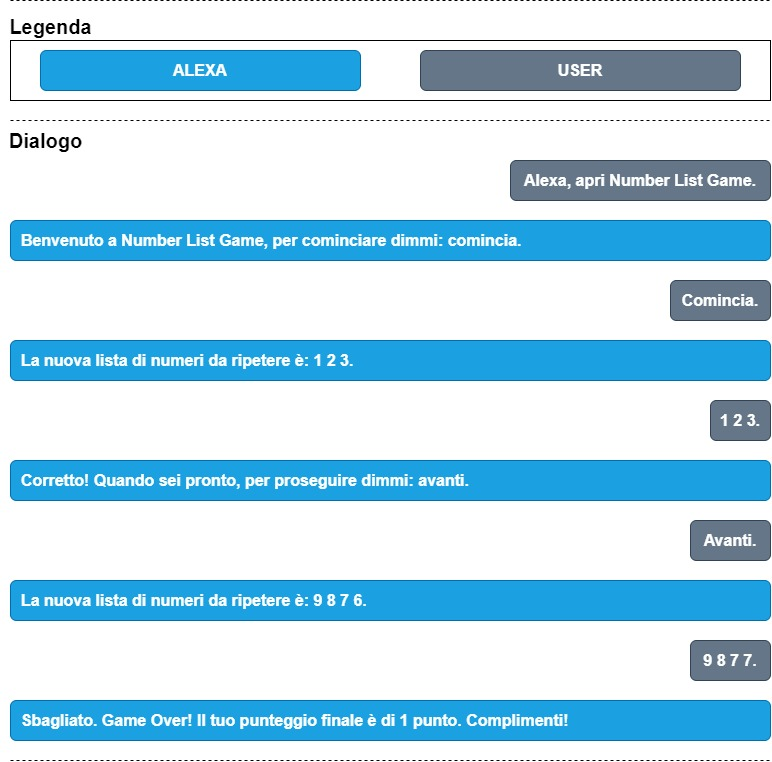
\includegraphics[scale=0.5]{resources/images/analysis/skill-flow-example/number-list-game-flow-example.jpg}
  \caption{
    Un esempio d'interazione con la \textit{skill} Number List Game,
    progettato per riassumere la logica del gioco.
  }
  \label{fig:figure4.1}
\end{figure}

\subsection{Progettazione del modello di dialogo}
\label{subsec:Sezione4.1.2}

Nel capitolo seguente, viene riportato il progetto di una possibile soluzione
che soddisfi i requisiti della \textit{skill} Number List Game. In particolare,
il progetto consiste in un diagramma di stati della \textit{skill}, in cui gli
stati sono da intendersi come \textbf{contesti} e \textbf{sotto-contesti}, in
cui ha senso esprimere una certa \textbf{intenzione} o meno. Il contesto in cui
si trova una \textit{skill} può cambiare in base alle intenzioni espresse
dall’utente. A ogni intenzione, corrisponde un’azione che sarà eseguita dalla
\textit{skill}.

\begin{figure}[!ht]
  \centering
  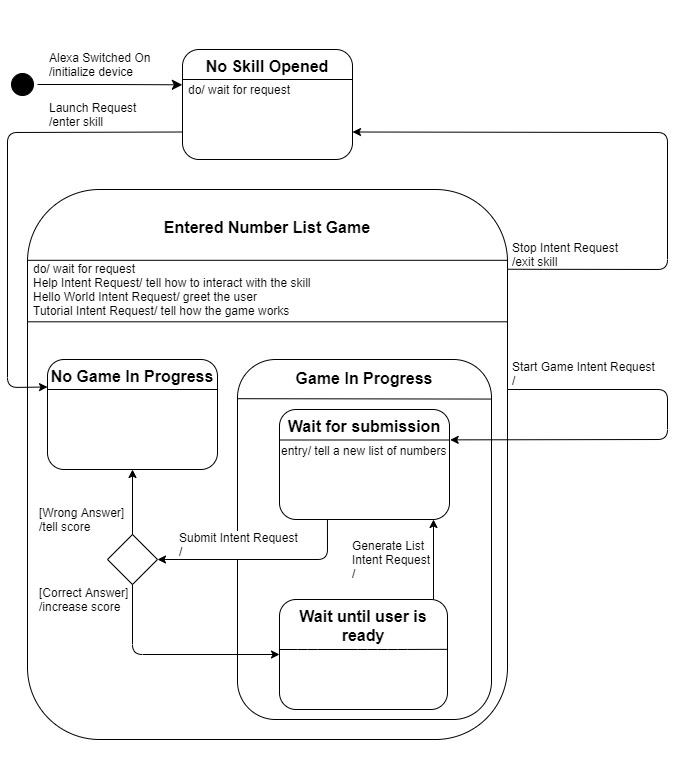
\includegraphics[scale=0.56]{resources/images/design/skill-state-diagram/number-list-game-state-diagram.jpg}
  \caption{Diagramma degli stati della \textit{skill} Number List Game.}
  \label{fig:figure4.2}
\end{figure}

Come si vede dalla Figura \ref{fig:figure4.2}, sarà possibile interagire con la
\textit{skill} attraverso le seguenti \textit{intenzioni}, all’interno degli
opportuni \textit{contesti} e \textit{sotto-contesti}:
\begin{itemize}
  \item \textbf{NO SKILL OPENED}: contesto in cui la skill non è ancora stata
        aperta; è anche il contesto in cui si trova Alexa subito dopo
        l’accensione:
        \begin{itemize}
          \item[o] \textit{\textbf{Launch Request}}: intenzione che esprime la
                volontà dell’utente di \textit{aprire la skill Number List
                Game};
        \end{itemize}
  \item \textbf{ENTERED NUMBER LIST GAME}: contesto in cui la skill è stata
        aperta:
        \begin{itemize}
          \item[o] \textit{\textbf{Stop Intent Request}}: intenzione che
                esprime la volontà dell’utente di \textit{uscire dalla skill
                Number List Game};
          \item[o] \textit{\textbf{Hello World Intent Request}}: intenzione che
                esprime la volontà dell’utente di \textit{essere salutato dalla
                skill Number List Game} (utilizzata per testare la
                comunicazione con la skill);
          \item[o] \textit{\textbf{Help Intent Request}}: intenzione che
                esprime la volontà dell’utente di \textit{conoscere com’è
                possibile interagire con la skill Number List Game};
          \item[o] \textit{\textbf{Tutorial Intent Request}}: intenzione che
                esprime la volontà dell’utente di \textit{conoscere come
                funziona il gioco};
          \item[o] \textit{\textbf{Start Game Intent Request}}: intenzione che
                esprime la volontà dell’utente di \textit{cominciare una nuova
                partita};
          \item[o] \textbf{NO GAME IN PROGRESS}: contesto in cui non è ancora
                stata cominciata nessuna partita;
          \item[o] \textbf{GAME IN PROGRESS}: contesto in cui è già in corso
                una partita:
                \begin{itemize}
                  \item[•] \textbf{WAIT FOR SUBMISSION}: contesto in cui la
                        skill ha comunicato una lista di numeri e aspetta che
                        l’utente la ripeti:
                        \begin{itemize}
                          \item[o] \textit{\textbf{Submit Intent Request}}:
                                intenzione che esprime la volontà
                                d'\textit{inviare una lista di numeri alla
                                skill};
                        \end{itemize}
                  \item[•] \textbf{WAIT UNTIL USER IS READY}: contesto in cui
                        la skill ha processato il tentativo corretto
                        dell’utente di ripetere la lista di numeri
                        precedentemente comunicata e aspetta una conferma da
                        parte del giocatore:
                        \begin{itemize}
                          \item[o] \textit{\textbf{Generate List Intent
                                Request}}: intenzione che esprime la volontà di
                                \textit{ricevere una nuova lista di numeri da
                                ripetere}.
                        \end{itemize}
                \end{itemize}
        \end{itemize}
\end{itemize}

\section{Category Game}
\label{sec:Sezione4.2}

Un altro gioco sviluppato per questa suite è \textbf{Category Game}. Il gioco
consiste nel categorizzare le parole comunicate da Alexa. In particolare,
possiede due diverse modalità:

\begin{itemize}
  \item[--] Nella \textit{modalità facile}, Alexa comunicherà al giocatore una
        categoria. Successivamente, a ogni turno, riferirà una parola diversa
        che il giocatore dovrà indicare come appartenente alla categoria o meno.
        Lo scopo della modalità è quello di allenare l’\textbf{attenzione} e la
        \textbf{categorizzazione}, infatti sarà richiesto all’utente di
        riconoscere solo alcune parole, tra tutte, come appartenenti a un
        certo gruppo;
  \item[--] Nella \textit{modalità difficile}, Alexa comunicherà al giocatore
        due categorie. Dopodiché, a ogni turno, riferirà una parola diversa
        appartenente a una delle due categorie menzionate. In questo caso però,
        il giocatore dovrà indicare la parola come appartenente alla categoria
        contraria a quella corretta.
        Lo scopo della modalità è quello di allenare l’\textbf{attenzione} e
        l’\textbf{inibizione degli automatismi}, infatti sarà richiesto
        all’utente di andare contro le sue abitudini e di rispondere in modo
        errato ai quesiti posti.
\end{itemize}

Il gioco termina al primo errore commesso dal giocatore, annunciando il suo
punteggio finale, ovvero il numero di parole che è riuscito a categorizzare
correttamente.

\subsection{Analisi del modello di dialogo}
\label{subsec:Sezione4.2.1}

Di seguito, viene riportata la progettazione di due esempi d'interazione tra
l’utente e la \textit{skill} Category Game, uno per modalità di gioco (Figura
\ref{fig:figure4.3} e Figura \ref{fig:figure4.4}). \newpage

\begin{figure}[!h]
  \centering
  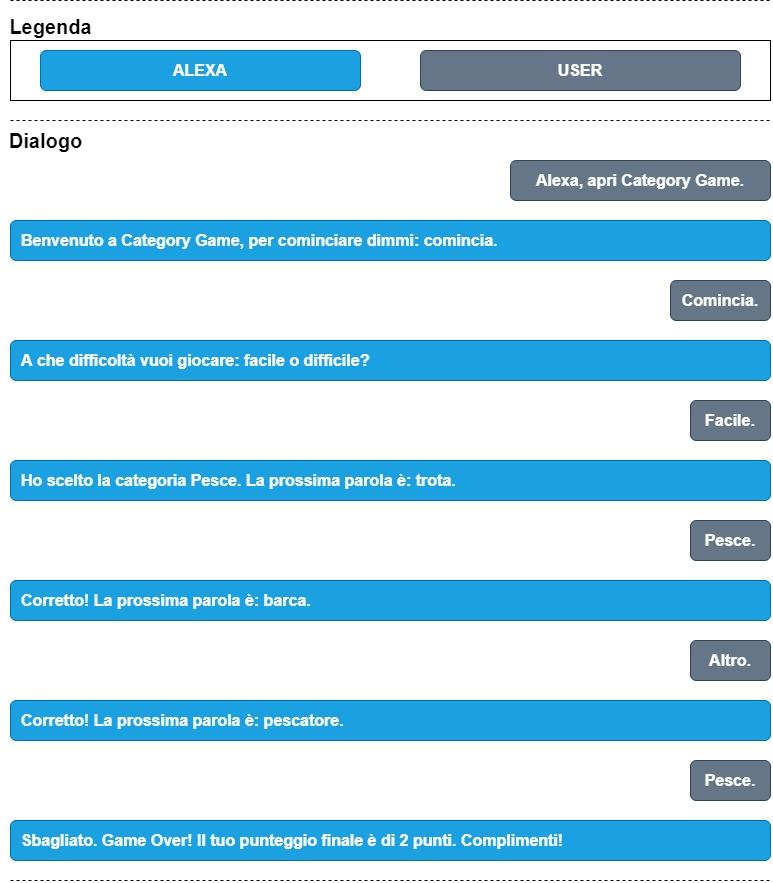
\includegraphics[scale=0.5]{resources/images/analysis/skill-flow-example/category-game-flow-example-easy.jpg}
  \caption{
    Esempio d'interazione con la \textit{skill} Category Game, progettato per
    riassumere la logica del gioco nella modalità facile.
  }
  \label{fig:figure4.3}
\end{figure}
\newpage

\begin{figure}[!h]
  \centering
  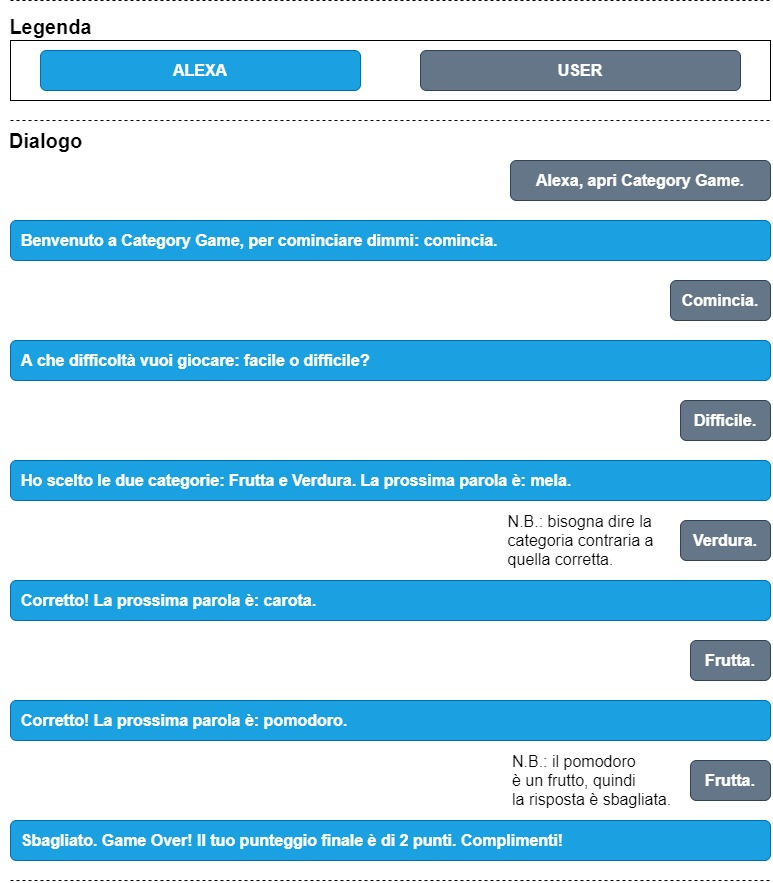
\includegraphics[scale=0.5]{resources/images/analysis/skill-flow-example/category-game-flow-example-difficult.jpg}
  \caption{
    Esempio d'interazione con la \textit{skill} Category Game, progettato per
    riassumere la logica del gioco nella modalità difficile.
  }
  \label{fig:figure4.4}
\end{figure}
\newpage

\subsection{Progettazione del modello di dialogo}
\label{subsec:Sezione4.2.2}

Ora viene riportato il progetto di una possibile soluzione che soddisfi i
requisiti della \textit{skill} Category Game.

\begin{figure}[!ht]
  \centering
  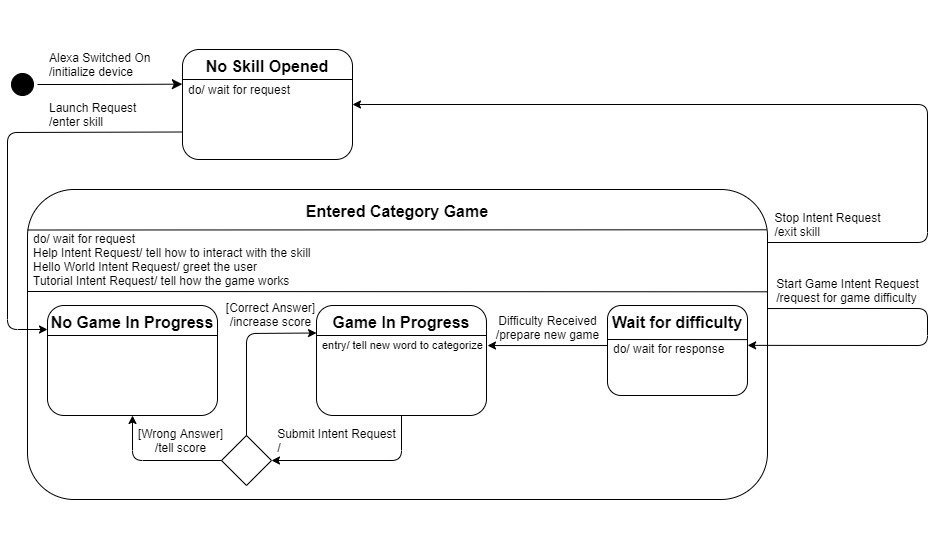
\includegraphics[scale=0.48]{resources/images/design/skill-state-diagram/category-game-state-diagram.jpg}
  \caption{Diagramma degli stati della \textit{skill} Category Game.}
  \label{fig:figure4.5}
\end{figure}

Come si vede dalla Figura \ref{fig:figure4.5}, sarà possibile interagire con la
\textit{skill} attraverso le seguenti \textit{intenzioni}, all’interno degli
opportuni \textit{contesti} e \textit{sotto-contesti}:
\begin{itemize}
  \item \textbf{NO SKILL OPENED}: contesto in cui la skill non è ancora stata
        aperta; è anche il contesto in cui si trova Alexa subito dopo
        l’accensione:
        \begin{itemize}
          \item[o] \textit{\textbf{Launch Request}}: intenzione che esprime la
                volontà dell’utente di \textit{aprire la skill Category Game};
        \end{itemize}
  \item \textbf{ENTERED NUMBER LIST GAME}: contesto in cui la skill è stata
        aperta:
        \begin{itemize}
          \item[o] \textit{\textbf{Stop Intent Request}}: intenzione che
                esprime la volontà dell’utente di \textit{uscire dalla skill
                Category Game};
          \item[o] \textit{\textbf{Hello World Intent Request}}: intenzione che
                esprime la volontà dell’utente di \textit{essere salutato dalla
                skill Category Game} (utilizzata per testare la comunicazione
                con la skill);
          \item[o] \textit{\textbf{Help Intent Request}}: intenzione che
                esprime la volontà dell’utente di \textit{conoscere com’è
                possibile interagire con la skill};
          \item[o] \textit{\textbf{Tutorial Intent Request}}: intenzione che
                esprime la volontà dell’utente di \textit{conoscere come
                funziona il gioco};
          \item[o] \textit{\textbf{Start Game Intent Request}}: intenzione che
                esprime la volontà dell’utente di \textit{cominciare una nuova
                partita}. In questo caso, prima di cominciare la partita, sarà
                richiesto all’utente di specificare anche la difficoltà a cui
                vuole giocare, che sarà utilizzata per determinare la modalità
                di gioco;
          \item[o] \textbf{NO GAME IN PROGRESS}: contesto in cui non è ancora
                stata cominciata nessuna partita;
          \item[o] \textbf{GAME IN PROGRESS}: contesto in cui è già in corso
                una partita ed è stata comunicata una parola da categorizzare
                al giocatore:
                \begin{itemize}
                  \item[•] \textit{\textbf{Submit Intent Request}}: intenzione
                        che esprime la volontà del giocatore
                        d'\textit{inviare una categoria alla skill}.
                \end{itemize}
        \end{itemize}
\end{itemize}

Si noti come in questo caso si sia deciso di non richiedere ogni turno la
conferma per proseguire nel gioco. Questa decisione è stata presa per
alleggerire il flusso di dialogo e diminuire il numero d'interazioni necessarie
per progredire in una partita.

\section{Labyrinth Game}
\label{sec:Sezione4.3}

\textbf{Labyrinth Game} è il gioco più complesso sviluppato per questa suite.

Il gioco consiste nel doversi muovere e orientare all’interno di un labirinto
bidimensionale, raggiungendone eventualmente l’uscita. All’inizio della
partita, Alexa genererà il labirinto. Successivamente, a ogni turno, Alexa
descriverà i dintorni del giocatore, il quale dovrà scegliere una direzione
verso cui spostarsi.

Come mostrato nella Figura \ref{fig:figure4.6}, il labirinto sarà composto di:
\begin{itemize}
  \item[--] \textit{Mura}: componenti non attraversabili;
  \item[--] \textit{Mura di perimetro}: componenti non attraversabili, che
        costituiscono il perimetro del labirinto;
  \item[--] \textit{Percorsi}: componenti attraversabili;
  \item[--] \textit{Torri}: componenti attraversabili, che forniscono dei
        suggerimenti al giocatore per aiutarlo a raggiungere l’uscita del
        labirinto;
  \item[--] \textit{Un’entrata}: il percorso su cui si trova il giocatore
        all’inizio della partita;
  \item[--] \textit{Un’uscita}: il percorso che dovrà raggiungere il giocatore
        per terminare la partita.
\end{itemize}
\begin{figure}[!ht]
  \centering
  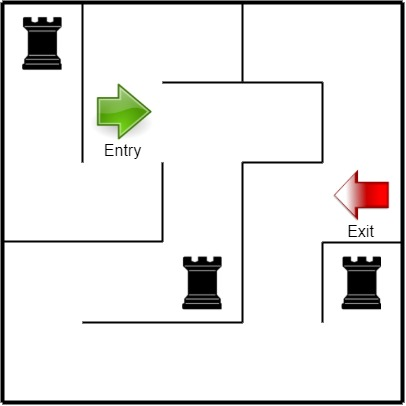
\includegraphics[scale=0.5]{resources/images/other/labyrinth-game-labyrinth-example.jpg}
  \caption{
    Esempio di layout di un labirinto nella \textit{skill} Labyrinth Game.
  }
  \label{fig:figure4.6}
\end{figure}

Il gioco termina quando il giocatore raggiunge l’uscita del labirinto,
annunciando il suo punteggio finale, ovvero il numero di passi che ha compiuto
prima di raggiungere l’uscita.

Lo scopo del gioco è quello di allenare la \textbf{memoria a lungo termine},
l’\textbf{orientamento} e l’\textbf{immaginazione}, infatti sarà richiesto
all’utente di ricordare e costruirsi mentalmente il layout del labirinto man
mano che lo esplora, riconoscendo la posizione in cui si trova.

\subsection{Analisi del modello di dialogo}
\label{subsec:Sezione4.3.1}

Di seguito, viene riportata la progettazione di un esempio d'interazione
dell’utente con la \textit{skill} Labyrinth Game (Figura \ref{fig:figure4.7}).
\newpage

\begin{figure}[!ht]
  \centering
  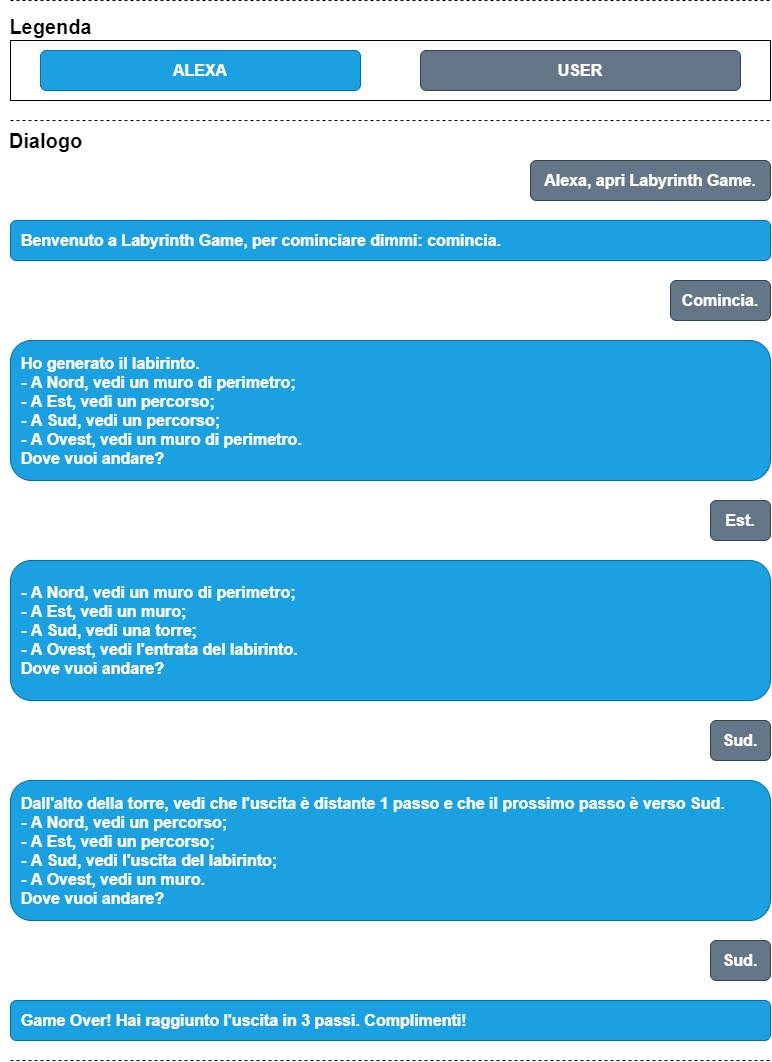
\includegraphics[scale=0.5]{resources/images/analysis/skill-flow-example/labyrinth-game-flow-example.jpg}
  \caption{
    Esempio d'interazione con la \textit{skill} Labyrinth Game, progettato per
    riassumere la logica del gioco.
  }
  \label{fig:figure4.7}
\end{figure}
\newpage

\subsection{Progettazione del modello di dialogo}
\label{subsec:Sezione4.3.2}

Ora viene riportato il progetto di una possibile soluzione che soddisfi i
requisiti della \textit{skill} Labyrinth Game.

\begin{figure}[!ht]
  \centering
  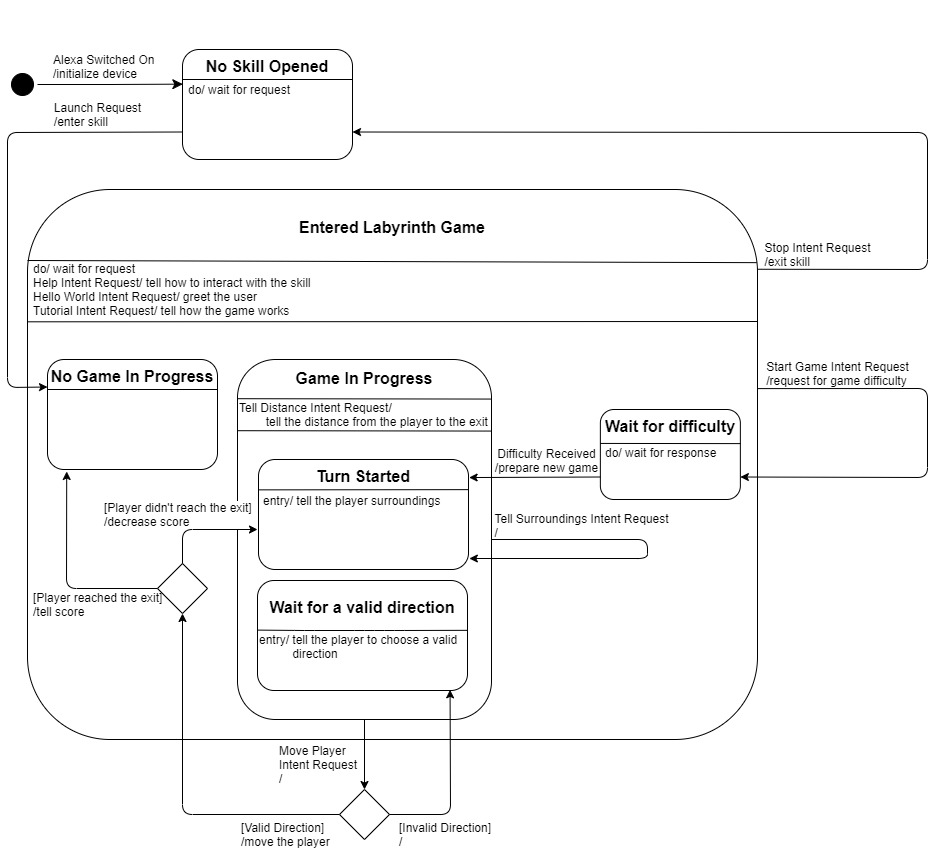
\includegraphics[scale=0.48]{resources/images/design/skill-state-diagram/labyrinth-game-state-diagram.jpg}
  \caption{Diagramma degli stati della \textit{skill} Labyrinth Game.}
  \label{fig:figure4.8}
\end{figure}

Come si vede dalla Figura \ref{fig:figure4.8}, sarà possibile interagire con la
\textit{skill} attraverso le seguenti \textit{intenzioni}, all’interno degli
opportuni \textit{contesti} e \textit{sotto-contesti}:
\begin{itemize}
  \item \textbf{NO SKILL OPENED}: contesto in cui la skill non è ancora stata
        aperta; è anche il contesto in cui si trova Alexa subito dopo
        l’accensione:
        \begin{itemize}
          \item[o] \textit{\textbf{Launch Request}}: intenzione che esprime la
                volontà dell’utente di \textit{aprire la skill Labyrinth Game};
        \end{itemize}
  \item \textbf{ENTERED NUMBER LIST GAME}: contesto in cui la skill è stata
        aperta:
        \begin{itemize}
          \item[o] \textit{\textbf{Stop Intent Request}}: intenzione che
                esprime la volontà dell’utente di \textit{uscire dalla skill
                Labyrinth Game};
          \item[o] \textit{\textbf{Hello World Intent Request}}: intenzione che
                esprime la volontà dell’utente di \textit{essere salutato dalla
                skill Labyrinth Game} (utilizzata per testare la comunicazione
                con la skill);
          \item[o] \textit{\textbf{Help Intent Request}}: intenzione che
                esprime la volontà dell’utente di \textit{conoscere com’è
                possibile interagire con la skill Labyrinth Game};
          \item[o] \textit{\textbf{Tutorial Intent Request}}: intenzione che
                esprime la volontà dell’utente di \textit{conoscere come
                funziona il gioco};
          \item[o] \textit{\textbf{Start Game Intent Request}}: intenzione che
                esprime la volontà dell’utente di \textit{cominciare una nuova
                partita}. Prima di cominciare la partita, sarà richiesto
                all’utente di specificare anche la difficoltà a cui vuole
                giocare, che sarà utilizzata per determinare le dimensioni del
                labirinto;
          \item[o] \textbf{NO GAME IN PROGRESS}: contesto in cui non è ancora
                stata cominciata nessuna partita;
          \item[o] \textbf{GAME IN PROGRESS}: contesto in cui è già in corso
                una partita ed è stato generato il labirinto su cui giocherà
                l’utente:
                \begin{itemize}
                  \item[•] \textit{\textbf{Tell Distance Intent}}: intenzione
                        che esprime la volontà del giocatore di
                        \textit{conoscere la sua distanza dall’uscita};
                  \item[•] \textbf{TURN STARTED}: contesto in cui sono già
                        stati descritti i dintorni del giocatore:
                        \begin{itemize}
                          \item[o] \textit{\textbf{Tell Surroundings Intent}}:
                                intenzione che esprime la volontà del giocatore
                                di \textit{conoscere i propri dintorni};
                          \item[o] \textit{\textbf{Move Player Intent}}:
                                intenzione che esprime la volontà del giocatore
                                di \textit{muoversi verso una certa direzione}.
                        \end{itemize}
                \end{itemize}
        \end{itemize}
\end{itemize}

A questo punto, una volta presentato il progetto, è possibile passare alla
descrizione della sua effettiva implementazione.
% ! TeX root = ../bachelor-thesis.tex

\chapter{Implementazione del prototipo}
\label{ch:Chapter5}

In questo capitolo, si discuterà l’implementazione prima del sistema domotico e
successivamente delle \textit{skill} di Alexa per gli esercizi cognitivi. In
entrambi i casi, saranno anche forniti degli esempi di codice che descriveranno
le interazioni tra le componenti di ciascun sistema.

\section{Implementazione del sistema domotico}
\label{sec:Sezione5.1}

In questa sezione, si illustrerà l’organizzazione del codice per il sistema
domotico e l’implementazione del servizio che permetterà all’utente di
controllare e monitorare i propri dispositivi domotici. Successivamente, sarà
fornito un esempio d'integrazione di un dispositivo domotico a OpenHAB, per il
quale è stata prevista la possibilità di una comunicazione bidirezionale tra
Alexa e OpenHAB.

\subsection{Struttura dei file di configurazione}
\label{subsec:Sezione5.1.1}

Di seguito, viene riportata la struttura standard dei file di configurazione di
OpenHAB (Figura \ref{fig:figure5.1}).

\begin{figure}[!ht]
  \centering
  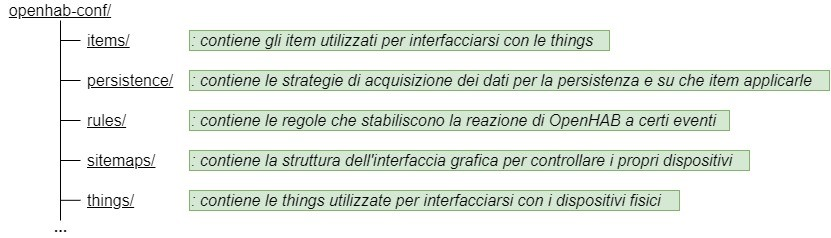
\includegraphics[scale=0.58]{resources/images/implementation/openhab-project-organization.jpg}
  \caption{
    L'organizzazione della directory che contiene i file di configurazione di
    OpenHAB.
  }
  \label{fig:figure5.1}
\end{figure}

I file di configurazione definiscono:

\begin{itemize}
  \item[--] \textit{Things} e \textit{Channels}: i dispositivi fisici connessi
        al sistema e le loro funzionalità;
  \item[--] \textit{Items}: i metodi e i componenti grafici utilizzabili per
        controllare i dispositivi, all’interno dei file di configurazione di
        OpenHAB e dell’interfaccia grafica rispettivamente;
  \item[--] \textit{Sitemaps}: l’organizzazione dei componenti nell’interfaccia
        grafica;
  \item[--] \textit{Rules}: le regole di automazione del sistema domotico,
        ovvero le sue reazioni agli eventi che riceve dai dispositivi che lo
        compongono;
  \item[--] \textit{Persistence}: le regole utilizzate per costruire uno
        storico degli stati degli item specificati.
\end{itemize}

Questi file sono caricati all’avvio della macchina in cui è stato installato
OpenHAB e a ogni loro aggiornamento durante l’esecuzione. Nel caso specifico,
il sistema domotico è stato installato su un \textbf{Raspberry PI}, con sistema
operativo a base \textbf{Linux}.

\subsection{Accesso al sistema domotico}
\label{subsec:Sezione5.1.2}

Per controllare il proprio sistema domotico è possibile accedere alla
\textbf{Dashboard di OpenHAB}, disponibile all’indirizzo IP della macchina su
cui è installato, su una specifica porta.

La dashboard permette di configurare il proprio sistema tramite interfaccia
grafica e d'interagire con le interfacce grafiche realizzate per controllare i
propri dispositivi domotici. In particolare, queste definiscono
l’organizzazione dei componenti grafici che potranno essere usati per
controllare i dispositivi domotici, ma non i componenti grafici stessi
(definiti invece dalle \textit{tipologie di item} usate per rappresentare le
funzionalità di quei dispositivi). I componenti grafici, oltre a controllare un
determinato dispositivo domotico, permettono di accedere allo storico dei suoi
stati in un certo periodo di tempo d’interesse.

Per controllare il sistema domotico, sono state rese disponibili due interfacce
grafiche:
\begin{itemize}
  \item[--] Una \textit{\textbf{sitemap}}: privilegia un’esposizione agevole e
        compatta delle funzionalità del sistema; quest’interfaccia era già stata
        predisposta in un tempo precedente rispetto a questo progetto;
  \item[--] Delle \textit{\textbf{pages}}: privilegiano l’estetica
        dell’interfaccia grafica.
\end{itemize}
Per le \textit{pages}, si è deciso di sfruttare una nuova funzionalità
introdotta nella versione 3.x di OpenHAB: il \textbf{modello semantico}.

Il modello semantico di un certo locale consente di organizzare logicamente i
propri dispositivi domotici, prima in base alla loro posizione nel locale e
successivamente in base alla loro funzionalità. OpenHAB è quindi in grado di:
\begin{itemize}
  \item[--] costruire il modello semantico automaticamente, se il codice
        rispecchia una certa struttura logica;
  \item[--] dal modello semantico, ricavare automaticamente un’interfaccia
        grafica ben strutturata, dalla quale è possibile controllare i propri
        dispositivi domotici.
\end{itemize}
Pertanto, è stato sufficiente riorganizzare la struttura di alcuni file di
configurazione, per ottenere un’interfaccia grafica già impostata, che
consentisse all’utente di controllare e monitorare il proprio sistema
domotico.

\subsection{Esempio d'integrazione con OpenHAB}
\label{subsec:Sezione5.1.3}

Ora sarà illustrato un esempio su come è possibile integrare una lampadina
Philips Hue al sistema domotico.

Innanzitutto, è necessario installare sul proprio sistema domotico un
\textit{add-on}, chiamato \textbf{Philips Hue Binding} \cite{BINDING_PH}.
Questo definirà alcune \textit{tipologie di thing}, che hanno \textit{channels}
preconfigurati per comunicare con dispositivi fisici della Philips Hue.

A questo punto è possibile iniziare a integrare i propri dispositivi domotici,
dichiarando le \textit{\textbf{things}} del sistema in un file
\textit{.things}.

\begin{figure}[!ht]
  \centering
  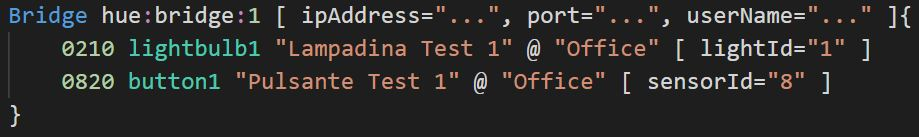
\includegraphics[scale=0.65]{resources/images/implementation/code/thing-code-example.jpg}
  \caption{
    Un esempio di file di configurazione per le \textit{thing}: in questo caso
    è stato dichiarato un bridge con due dispositivi connessi, una lampadina e
    un pulsante.
  }
  \label{fig:figure5.2}
\end{figure}

Nell’esempio (Figura \ref{fig:figure5.2}), viene integrato un \textbf{bridge
Hue} a cui sono collegati una \textbf{lampadina} e un \textbf{pulsante} della
Philips Hue. Queste sono le \textit{things} vere e proprie e sono
contraddistinte da due proprietà principali:
\begin{itemize}
  \item[--] Il \textit{\textbf{tipo di thing}}, che dichiara i \textit{channel}
        disponibili a quella \textit{thing}, ovvero le funzionalità del
        dispositivo. In questo caso, sono forniti dal \textit{binding} del
        produttore specifico (nell’esempio: \textit{0210} e \textit{0820});
  \item[--] Il \textit{\textbf{nome della thing}}, che serve per riconoscerla
        all’interno dei file di configurazione di OpenHAB (nell’esempio:
        \textit{lightbulb1} e \textit{button1}).
\end{itemize}

Una volta integrati i dispositivi domotici al sistema OpenHAB, bisogna definire
come sarà possibile controllarli nei file di configurazione e nell’interfaccia
grafica, dichiarando gli \textit{\textbf{items}} del sistema in un file
\textit{.items}.

\begin{figure}[!ht]
  \centering
  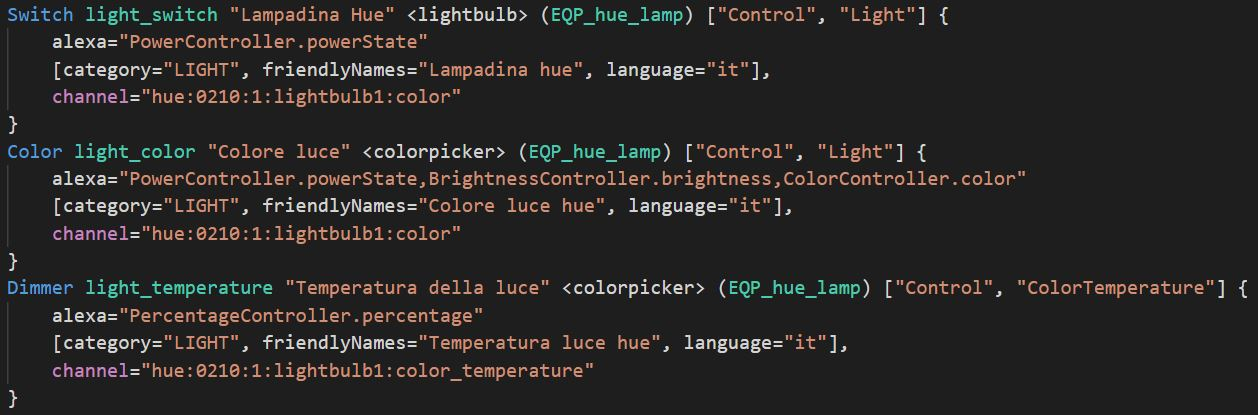
\includegraphics[scale=0.48]{resources/images/implementation/code/items-code-example.jpg}
  \caption{
    Un esempio di file di configurazione per gli \textit{items}: in questo caso
    sono state esposte le funzionalità di una lampadina Hue, che comprendono
    l'accensione, il colore e la temperatura del colore.
  }
  \label{fig:figure5.3}
\end{figure}

Nell’esempio (Figura \ref{fig:figure5.3}) sono stati creati tre \textit{items}
per la lampadina integrata precedentemente: uno \textbf{Switch} per accendere e
spegnere la lampadina, un \textbf{Color} per impostarne il colore e un
\textbf{Dimmer} per regolarne la temperatura del colore. I punti focali della
sintassi di un \textit{item} sono:
\begin{itemize}
  \item[--] Il \textit{\textbf{tipo di item}}, che definisce come sarà
        possibile interagire con le funzionalità che controlla. I \textit{tipi
          di item} sono standard e ognuno fornisce gli stati che può assumere
        l’\textit{item} e i comandi che può ricevere. Ad esempio, uno Switch
        può essere acceso (\textit{ON}) o spento (\textit{OFF});
  \item[--] Il \textit{\textbf{nome dell’item}}, che serve per riconoscerlo
        all’interno dei file di configurazione di OpenHAB (nell’esempio
        \textit{light\_switch}, \textit{light\_color} e
        \textit{light\_temperature});
  \item[--] Il \textit{\textbf{channel associato}}, che definisce le
        funzionalità che l’\textit{item} controlla e il ponte tra
        \textit{item} e \textit{thing}. In questo caso, la sintassi usata per
        identificare un \textit{channel} è definita dal \textit{binding} a cui
        appartiene, ovvero Philips Hue Binding (nell’esempio:
        \textit{channel=”hue:0210:1:lightbulb1:color”} permette di controllare
        il colore e lo stato di accensione della \textit{thing}
        \textit{lightbulb1}).
  \item[--] L’\textit{\textbf{interfaccia di Alexa implementata}}, che serve
        per configurare la \textbf{skill di OpenHAB} per Alexa. In particolare,
        indica con quali comandi vocali si potrà controllare
        quell’\textit{item} attraverso un dispositivo Alexa (nell’esempio:
        \textit{alexa= ”PowerController.PowerState” […]}).
\end{itemize}

A questo punto è già possibile controllare i propri dispositivi domotici
tramite Alexa e, assumendo che la sintassi rispetti le regole del modello
semantico di OpenHAB, anche attraverso un'interfaccia grafica, generata
automaticamente, su OpenHAB.

L’ultima cosa che rimane da fare, è quella di notificare l’utente degli eventi
rilevati da OpenHAB. A questo proposito, sarà necessario installare un altro
\textit{add-on} sul proprio sistema domotico: \textbf{Amazon Echo Control
Binding}. Questo \textit{binding} permetterà d'integrare un dispositivo Alexa a
OpenHAB, con un metodo analogo a quello utilizzato per la lampadina Hue.
Dunque, sarà possibile controllarlo attraverso una regola di automazione,
definendo una \textit{\textbf{rule}} in un file \textit{.rules}.

\begin{figure}[!ht]
  \centering
  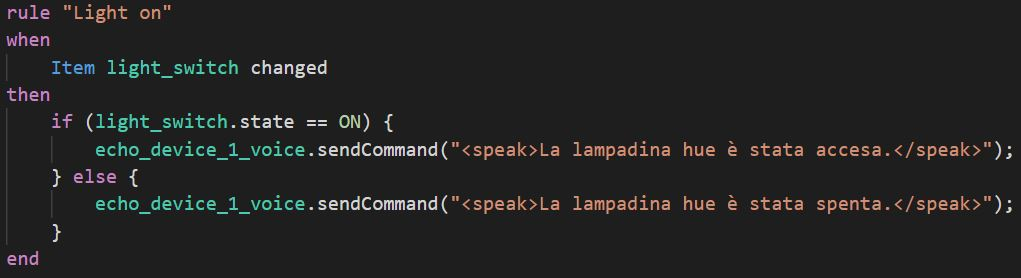
\includegraphics[scale=0.59]{resources/images/implementation/code/rule-code-example.jpg}
  \caption{
    Un esempio di file di configurazione per le \textit{rules}: in questo caso
    è stato definito un \textit{handler} che reagisce ai cambiamenti di stato
    della lampadina Hue, comunicandoli all'utente tramite un dispositivo Alexa.
  }
  \label{fig:figure5.4}
\end{figure}

Nell’esempio (Figura \ref{fig:figure5.4}), viene definita una regola che
risponde ai cambiamenti dello stato di accensione della lampadina Hue (ovvero
se è stata accesa o spenta), controllando un dispositivo Alexa Echo e quindi
comunicando all’utente il nuovo stato della lampadina.

\section{Implementazione delle skill}
\label{sec:Sezione5.2}

In questa sezione, si illustrerà l’organizzazione del codice per il progetto
del servizio che espone gli esercizi cognitivi e l’implementazione
dell’interazione tra l’utente e tale servizio. Infine, saranno presentati
alcuni estratti di codice che aiutino a visualizzare nel concreto le componenti
del sistema e le loro interazioni.

Per l’implementazione è stato utilizzato il linguaggio di programmazione
\textbf{TypeScript} \cite{TYPESCRIPT}, che è un’estensione tipizzata di
\textbf{JavaScript}. Il servizio è stato costruito sul framework
\textbf{node.js} \cite{NODE.JS}, il cui scopo è gestire applicazioni di rete
scalabili, e in particolare sul framework \textbf{Express} \cite{EXPRESS},
utilizzato per costruire applicazioni web.

\subsection{Struttura dell'applicazione}
\label{subsec:Sezione5.2.1}

Di seguito, viene riportata la struttura organizzativa utilizzata nella
directory del progetto sugli esercizi cognitivi (Figura \ref{fig:figure5.5}).
Sono quindi evidenziate, le componenti principali del progetto e la loro
funzione.

\begin{figure}[!ht]
  \centering
  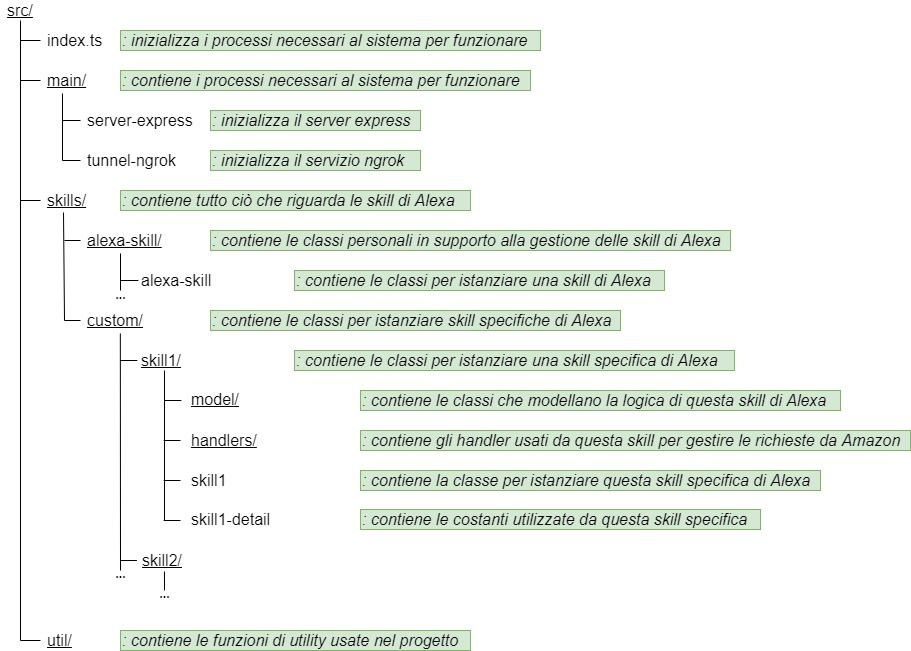
\includegraphics[scale=0.58]{resources/images/implementation/alexa-project-organization.jpg}
  \caption{
    L'organizzazione della directory che contiene l'applicazione che gestisce
    il servizio per le \textit{skill} cognitive.
  }
  \label{fig:figure5.5}
\end{figure}

\subsection{Funzionamento dell'applicazione}
\label{subsec:Sezione5.2.2}

All’avvio, l’applicazione crea il \textbf{server Express} utilizzato per
accedere al servizio. Questo potrà ricevere le \textit{richieste http}
dell’utente, delegandone la gestione ad alcuni \textit{handler}, selezionati in
base al \textit{percorso} specificato dall’utente. Successivamente, viene
verificata l’esistenza di un \textbf{tunnel ngrok} verso la porta del
\textit{server Express}: se non è presente, viene avviato un nuovo processo,
che eseguirà \textit{ngrok} in modo indipendente dall’applicazione. Il processo
\textit{ngrok} dovrà rimanere attivo anche dopo la chiusura dell’applicazione,
così non sarà riavviato insieme all’applicazione. Infatti, per inizializzare
l’applicazione, è stato utilizzato il processo \textit{Nodemon} per Node.js,
che, una volta avviato, rileva ogni aggiornamento sulla directory indicatagli,
reagendo con un riavvio automatico dell’applicazione, quindi applicando le
modifiche eseguite sul codice.

All’inizializzazione del \textit{server Express}, vengono anche creati i
gestori delle richieste http. Questi consistono nelle vere e proprie
\textbf{skills di Alexa}. Ogni \textit{skill} viene associata al \textit{server
Express} su uno specifico percorso, tramite un \textbf{Express Adapter}, che si
occuperà di validare le richieste http in entrata, controllando che
effettivamente provengano da Amazon Alexa.

Una \textit{skill} avrà il compito di gestire tutte le richieste http sul
percorso assegnatole. Più in dettaglio, riceverà tutte le \textit{intenzioni}
dell’utente che le competono e le smisterà verso gli opportuni \textbf{intent
handlers}. Ogni \textit{intent handler} gestirà una specifica intenzione
dell’utente, interagendo con il \textbf{modello della skill}, che contiene le
classi che descrivono la logica del gioco cognitivo implementato. Al termine
dell’esecuzione, un \textit{intent handler} produrrà un’opportuna risposta, che
sarà comunicata mediante il dispositivo Alexa.

I progressi di un relativo giocatore durante il gioco, vengono memorizzati
sulle variabili di sessione della \textit{skill}, chiamate
\textit{\textbf{session attributes}}. La sessione di una certa \textit{skill} è
relativa all’interazione con uno specifico utente e viene creata all’apertura
della \textit{skill}, permanendo fino alla sua chiusura. Specificamente, è
mantenuta all’interno dei messaggi scambiati tra l’utente e il servizio.

Di seguito, viene riportato uno schema che riassume i componenti descritti
precedentemente (Figura \ref{fig:figure5.6}).
\begin{figure}[!ht]
  \centering
  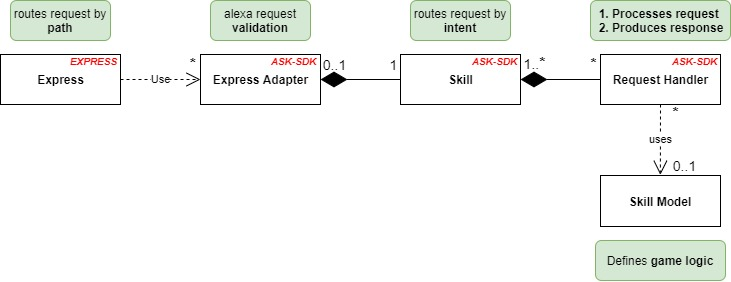
\includegraphics[scale=0.6]{resources/images/implementation/project-class-diagram.jpg}
  \caption{
    Schema che descrive i componenti principali dell'applicazione in base alla
    loro funzione.
  }
  \label{fig:figure5.6}
\end{figure}

Al termine dell’avvio, il \textit{server Express} mostrerà le caratteristiche
del servizio, come mostrato in Figura \ref{fig:figure5.7} (da notare che il
caricamento del server impiega molto tempo quando il servizio \textit{ngrok}
non è già in esecuzione).

Siccome l’indirizzo pubblico del proprio servizio cambia a ogni esecuzione di
\textit{ngrok} (nella licenza gratuita), è necessario ricordarsi di mantenere
aggiornati gli \textit{\textbf{endpoint}} utilizzati dalle \textit{skill}. Gli
\textit{endpoint} sono modificabili dal modello di dialogo delle
\textit{skill}, accessibile dall’\textit{Alexa Skills Kit} dell’\textit{Amazon
Developer Console}. Nella figura, questi endpoint hanno gli indirizzi URL
mostrati nella sezione \textit{LOADED SKILLS}.

\begin{figure}[!ht]
  \centering
  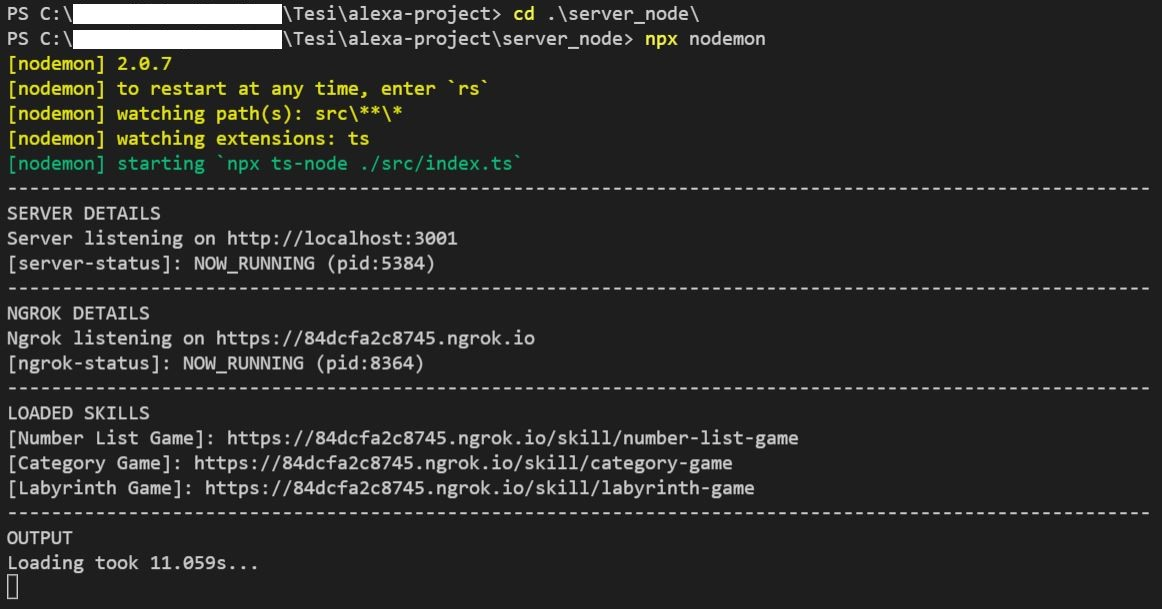
\includegraphics[scale=0.5]{resources/images/implementation/code/express-server-starting-capture.jpg}
  \caption{
    Output del \textit{server Express} dopo la sua inizializzazione. Di
    particolare importanza è la sezione \textit{LOADED SKILLS}.
  }
  \label{fig:figure5.7}
\end{figure}

Una volta finita la configurazione, il servizio è pronto per essere acceduto da
un qualsiasi dispositivo Alexa, che sia associato a un account Amazon in cui
sono installate le \textit{skill}. Siccome non è ancora stato eseguito il
deployment delle \textit{skill}, queste saranno accessibili solo dall’account
che le sta sviluppando.

\subsection{Esempio d'implementazione di una skill}
\label{subsec:Sezione5.2.3}

Ora sarà illustrato un esempio su come è possibile implementare una
\textit{skill}, raggiungibile attraverso un server realizzato con
\textit{Express}.

Inizialmente, è necessario configurare il \textbf{server Express} (Figura
\ref{fig:figure5.8}). Ciò significa creare le \textbf{skills} che dovrà gestire
e mapparle a un determinato percorso nel server. Siccome, su quei percorsi si
vuole accettare solo richieste provenienti da Alexa, viene utilizzato un
\textbf{Express Adapter}, il cui scopo è modificare gli \textit{handler} di una
\textit{skill}, in modo che eseguano una verifica sulla sorgente della
richiesta, preliminarmente alla sua gestione. Il \textit{server Express} si
occuperà di smistare le richieste in entrata in base al percorso da loro
indicato, delegandole alla \textit{skill} opportuna.

\begin{figure}[!ht]
  \centering
  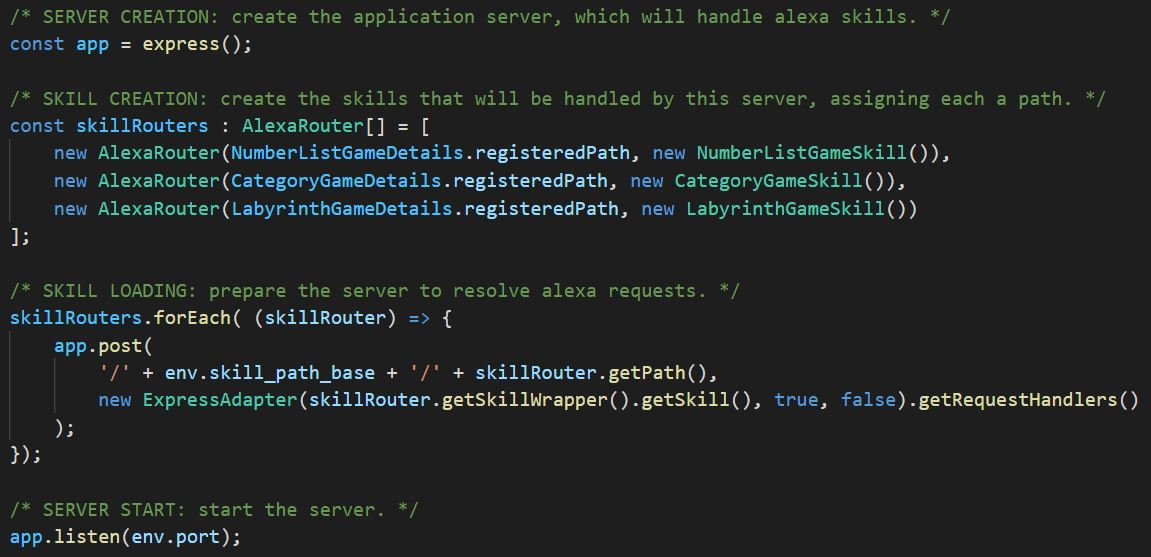
\includegraphics[scale=0.52]{resources/images/implementation/code/server-start-code-example.jpg}
  \caption{
    Inizializzazione del \textit{server Express}. Include la creazione delle
    \textit{skill} e la loro mappatura sul server.
  }
  \label{fig:figure5.8}
\end{figure}

\begin{figure}[!ht]
  \centering
  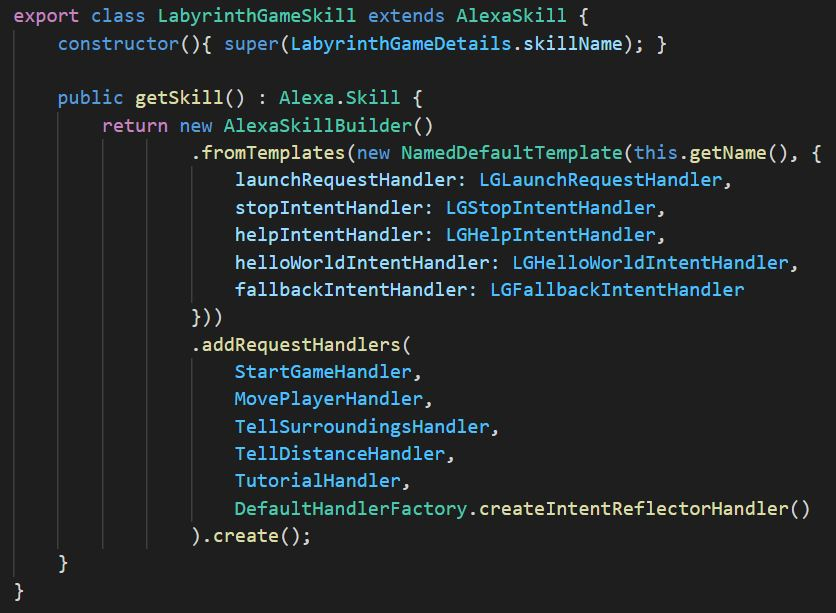
\includegraphics[scale=0.52]{resources/images/implementation/code/skill-code-example.jpg}
  \caption{
    Inizializzazione di una \textit{skill}. Qui sono inizializzati tutti
    gli \textit{intent handler} utilizzati dalla \textit{skill}.
  }
  \label{fig:figure5.9}
\end{figure}

La creazione di una \textit{skill} (Figura \ref{fig:figure5.9}) avviene
attraverso uno \textbf{Skill Builder}, che ne determina gli \textit{handler}.
Lo \textit{Skill Builder} utilizzato è un’estensione di quello fornito dalla
libreria \textbf{ASK-SDK} e distingue gli handler in due categorie:
\begin{itemize}
  \item[--] Gli \textit{handler standard}, che sono molto simili tra le varie
        \textit{skill}, quindi si prestano bene a essere raggruppati in un
        \textbf{template}, applicabile su \textit{skill} diverse. Ad esempio,
        sono considerati standard gli \textit{handler} indicati da Amazon come
        necessari al deployment di una \textit{skill};
  \item[--] Gli \textit{handler custom} che caratterizzano una specifica
        \textit{skill}, in base alle funzionalità che offre.
\end{itemize}
Ogni \textit{skill} si occuperà di gestire le richieste su di uno specifico
percorso del server in base all’intenzione espressa dall’utente, delegandole
all’\textit{handler} opportuno.

Gli \textit{handler di una skill} sono caratterizzati da due metodi principali
(Figura \ref{fig:figure5.10}). Una funzione, chiamata
\textit{\textbf{canHandle}}, permette alla \textit{skill} di verificare se
l’\textit{handler} può gestire una certa richiesta. Una volta verificato ciò,
può essere applicata la seconda funzione, chiamata \textit{\textbf{handle}},
che gestisce la richiesta. Gli \textit{handler} interagiranno con il modello
della \textit{skill}, controllando il progresso nel gioco, la cui logica è
definita nel modello stesso. Il progresso nel gioco sarà memorizzato nei
parametri della sessione attiva tra l’utente e la \textit{skill} specifica.

\begin{figure}[!ht]
  \centering
  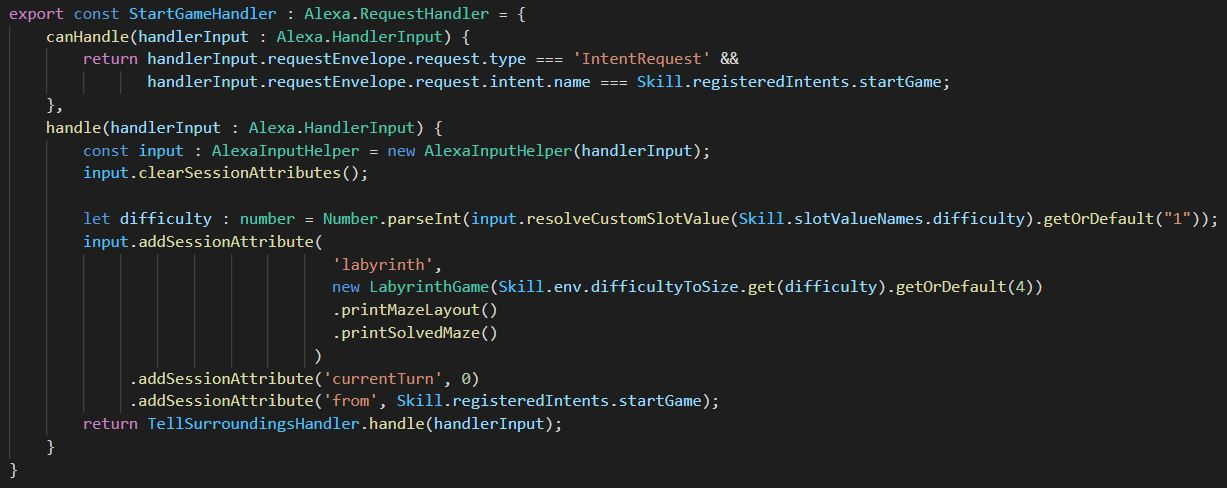
\includegraphics[scale=0.49]{resources/images/implementation/code/skill-handler-code-example.jpg}
  \caption{
    Esempio d'implementazione di un \textit{intent handler}. Si notano i
    caratteristici metodi di un intent handler e l'interazione con il modello
    della skill (ovvero la classe \textit{LabyrinthGame}).
  }
  \label{fig:figure5.10}
\end{figure}

Normalmente, un \textit{handler} produce anche una risposta, che sarà
comunicata dal dispositivo Alexa. Nell’esempio però, la generazione della
risposta è delegata a un altro \textit{handler} della \textit{skill}.

% ! TeX root = ../bachelor-thesis.tex

\chapter{Validazione del sistema}
\label{ch:Chapter6}

In questo capitolo, si descriveranno i metodi utilizzati per validare
l'applicazione, ovvero i test che sono stati eseguiti per verificarne la
correttezza e l’adeguatezza rispetto i requisiti preposti.

\section{Metodi di validazione}
\label{sec:Section6.1}

Al tempo della scrittura di questo elaborato, viste anche le limitazioni legate
all'emergenza \textit{COVID-19}, non era ancora stato possibile eseguire delle
prove che coinvolgessero il target dell'applicazione. Questi test sugli utenti
finali sono necessari ancor di più nel contesto della \textit{gamification},
quindi saranno sicuramente eseguiti in futuro.

Per il momento, nondimeno, sono stati eseguiti numerosi \textit{friendly-trial}
in ambiente chiuso all’interno del CRA di Bologna. Nello specifico, sono state
eseguite delle prove che verificassero:
\begin{itemize}
  \item[--] La \textit{\textbf{possibilità di controllare i dispositivi
            domotici attraverso OpenHAB}}; per questo è stata utilizzata
        l’interfaccia grafica costruita, accertandosi che a un comando
        dell'utente corrispondesse una reazione adeguata del sistema
        domotico (ad esempio, in riferimento alle figure
        \ref{fig:figure5.2} e \ref{fig:figure5.3}, alla pressione del
        pulsante \textit{light\_switch}, la lampadina \textit{lightbulb1}
        si deve accendere o spegnere);
  \item[--] La \textit{\textbf{possibilità di controllare i dispositivi
            domotici con dei comandi vocali attraverso Alexa}}; per questo è
        stata utilizzata la skill di OpenHAB attraverso Alexa, accertandosi che
        a un comando vocale dell'utente corrispondesse una reazione adeguata
        del sistema domotico (ad esempio, in riferimento alle figure
        \ref{fig:figure5.2} e \ref{fig:figure5.3}, dicendo ad Alexa
        \textit{"Accendi / Spegni la Lampadina Hue"}, la lampadina
        \textit{lightbulb1} si deve accendere o spegnere);
  \item[--] La \textit{\textbf{capacità di OpenHAB di notificare l’utente di
            certi eventi relativi ai dispositivi domotici connessi}}; per
        questo sono stati generati degli eventi nel sistema domotico,
        accertandosi che questi fossero comunicati correttamente attraverso
        Alexa (ad esempio, in riferimento alla figura \ref{fig:figure5.4},
        Alexa deve comunicare quando la lampadina \textit{lightbulb1} viene
        accesa o spenta);
  \item[--] L'\textit{\textbf{adeguatezza delle skill nell’esercitare le
            capacità cognitive dell’utente}}; per questo si è lasciato giocare
        alcuni utenti che non fossero direttamente coinvolti
        nell'implementazione delle \textit{skill}, prendendo atto delle
        recensioni e del feedback ricevuto, così da effettuare cambiamenti che
        ne migliorassero l'usabilità.
\end{itemize}
Il funzionamento del sistema è stato testato da alcuni membri del personale del
CRA di Bologna. Nello specifico, i risultati ottenuti sul sistema domotico e
sulle \textit{skill} di Alexa sono stati approvati da alcuni componenti del
team multidisciplinare del CRA, tra cui la neuropsicologa \textit{Dott.ssa
  Arianna Gherardini}, e i correlatori \textit{Ing. Massimiliano Malavasi},
coordinatore del CRA, e \textit{Dott.ssa Laura Bugo}, sviluppatrice software.

\section{Risultati ottenuti}
\label{sec:Section6.2}

Di seguito, saranno riportati e commentati i risultati ottenuti dai test
eseguiti sul sistema domotico e sulle \textit{skill} implementate.

\subsection{Il sistema domotico}
\label{subsec:Section6.2.1}

Il funzionamento del sistema domotico si è rilevato adeguato e soddisfacente.
Tuttavia, è possibile fare alcuni commenti sulle responsività constatate nelle
diverse interazioni rese disponibili all'utente.

L'\textit{interazione attraverso l'interfaccia grafica} è quella con minor
latenza. Ciò ha senso se si tiene conto del fatto che i comandi inviati tramite
interfaccia grafica sono inviati a OpenHAB senza intermediari. Maggiore è
invece la latenza delle \textit{interazioni vocali attraverso Alexa}. In questo
caso, i comandi devono essere interpretati dal cloud di Alexa, per questo
trascorrono un paio di secondi prima che l'utente possa osservare un riscontro
sul sistema domotico. Considerando che lo scopo dell'integrazione con Alexa era
in primo luogo di fornire ulteriori strumenti accessibili per controllare il
proprio sistema domotico, i tempi di risposta ottenuti sono stati valutati come
accettabili. Altrettanta latenza si è stata constatata nella \textit{ricezione
delle notifiche} sugli eventi accaduti nel sistema domotico. Questa funzione
era stata pensata per ricordare all'utente alcuni compiti da svolgere, a orari
prestabiliti, in base allo stato del sistema domotico (come ricordare
all'utente di chiudere le finestre d'inverno prima di dormire, se ce n'è
qualcuna aperta). Qualche secondo di differenza rispetto a tali orari, non
influenza il risultato finale, quindi anche in questo caso si è ritenuto il
sistema soddisfacente.

\subsection{Number List Game}
\label{subsec:Section6.2.2}

Riguardo alla \textit{skill} Number List Game, sono stati ricevuti alcuni
feedback costruttivi, soprattutto riguardo ad alcuni problemi di progettazione.
Nel complesso, è stato un buon primo tentativo d'implementazione di una
\textit{skill} per Alexa.

I feedback ricevuti riguardano soprattutto il flusso di dialogo. Infatti, la
\textit{skill} richiede una conferma ogni volta che l'utente invia la risposta
al quesito precedentemente comunicato da Alexa. Considerando che, nelle
interazioni con una \textit{skill}, ovvero con il cloud, esiste anche una certa
latenza, ciò può diventare abbastanza tedioso per il giocatore. Nelle
\textit{skill} progettate successivamente, si è dunque deciso di snellire il
modello di dialogo, raggiungendo gli stessi risultati attraverso meno
interazioni.

\subsection{Category Game}
\label{subsec:Section6.2.3}

La \textit{skill} Category Game ha ricevuto feedback molto positivi. Non
significa però, che non possano ancora essere migliorati alcuni suoi aspetti.

Il problema principale è la mancanza di contenuti. In effetti, la
\textit{skill} necessita di una maggiore varietà di categorie e di parole
conosciute: capita spesso che sia richiesto all'utente di categorizzare la
stessa parola in un breve periodo di tempo, oppure di fare partite consecutive
in cui siano coinvolte le stesse categorie. Siccome le categorie e le parole
sono definite in modo statico, una soluzione potrebbe essere l'aggiornamento
dei file che le contengono, o ancora meglio, se possibile, richiederle a
servizi terzi che già gestiscono dati simili.

\subsection{Labyrinth Game}
\label{subsec:Section6.2.4}

Labyrinth Game è stato un esperimento che ha avuto abbastanza successo. In fase
di progettazione, si pensava infatti che sarebbe stato troppo difficile per
l'utente seguire il flusso di dialogo del gioco e pertanto interagire con la
\textit{skill}. Tuttavia, si è scoperto invece che ci si abitua velocemente
alla struttura con cui si riferiscono le informazioni nel gioco. Dunque, già
all'interno della prima partita, le difficoltà iniziali vengono riscontrate
sempre meno.

Questi risultati sono stati ottenuti dopo alcune fasi di raffinamento, in cui
lo scopo principale era di bilanciare il dialogo tra l'utente e Alexa: in
questo tipo di gioco, l'utente riceve molte più informazioni rispetto a quelle
che fornisce. Per agevolare la concentrazione dell'utente, si è quindi cercato
di essere il più possibile concisi e schematici nel riferirgli le informazioni
necessarie per giocare, così da rendere il dialogo più interattivo.

% ! TeX root = ../bachelor-thesis.tex

\chapter*{Conclusioni}
\addcontentsline{toc}{chapter}{Conclusioni}

In questo elaborato si è cercato d'illustrare al meglio le caratteristiche di
un sistema che potesse soddisfare i requisiti funzionali preposti. Il risultato
è stato nel complesso adeguato e soddisfacente, ma possono essere fatte alcune
considerazioni finali.

In primo luogo, il sistema è ancora in fase prototipale e saranno necessari
alcuni raffinamenti. Nello specifico, per quanto riguarda il sistema domotico,
sarà necessario cercare di migliorarne la reattività. Ciò dipende in gran parte
dalle tecnologie utilizzate, quindi si dovrà mantenere il sistema aggiornato,
in modo da adottare le nuove funzionalità e i miglioramenti che queste
offriranno. Per quanto riguarda le \textit{skill} implementate, sarà invece
necessario continuare a perfezionarne il modello di dialogo, rendendo sempre
più agevoli e interessanti le interazioni con Alexa.

In secondo luogo, il sistema dovrà essere verificato non solo in ambiente
chiuso, ma anche attraverso il coinvolgimento di un campione del target
indicato. Questo risulterà necessario per dimostrare l'effettiva adeguatezza
del sistema, soprattutto per gli esercizi cognitivi implementati.

In futuro, il progetto potrà essere esteso ed essere integrato in un contesto
socio-sanitario, nel quale potrà sperabilmente assistere persone con disabilità
o difficoltà cognitive a raggiungere una maggiore indipendenza.

In conclusione, si spera che questo progetto possa essere ultimato, producendo
tutti i risultati desiderati, e che possa concretamente assistere altre
persone, offrendo loro l'opportunità di ottenere una maggiore libertà.

% ! TeX root = ../bachelor-thesis.tex

\chapter*{Ringraziamenti}
\addcontentsline{toc}{chapter}{Ringraziamenti}

Ringrazio,\\

\textit{la mia famiglia e i miei genitori, per avermi supportato in questo
  percorso, permettendomi di proseguire con gli studi e offrendomi questa
  opportunità per crescere, ma anche per avermi insegnato a essere indipendente
  e sostenuto nella mia ricerca d'indipendenza;}\\

\textit{i miei amici, per le esperienze e le conoscenze condivise, i loro
  diversi punti di vista e le discussioni anche scherzosamente animate, ma
  sicuramente costruttive;}\\

\textit{i membri del team del CRA di Bologna, per avermi ospitato
  calorosamente, aiutato a integrarmi nell'ambiente di lavoro e formato negli
  argomenti trattati dalla tesi; in particolare, il tutor aziendale e correlatore
  della tesi, Ing. Massimiliano Malavasi, e la correlatrice, Dott.ssa Laura Bugo,
  che mi hanno seguito nello sviluppo del progetto; inoltre, la neuropsicologa
  Dott.ssa Arianna Gherardini, per avermi formato e assistito nella
  progettazione dei giochi cognitivi;}\\

\textit{i professori universitari, per offrire l'opportunità d'intraprendere
  questo tipo di percorso didattico e formativo; in particolare, il professore
  Alessandro Ricci, che mi ha introdotto alla gestione della comunicazione tra
  sistemi diversi e poi seguito nella stesura di questa stessa tesi.}\\

Grazie a tutti voi.

\backmatter

\bibliography{bibliography}{}
\bibliographystyle{unsrt}

\end{document}